%\documentclass{report}
%\usepackage[T1]{fontenc}
%\usepackage[utf8]{inputenc}
%\usepackage[francais]{babel}
%\usepackage{amsmath}
%\usepackage{graphicx}
%\graphicspath{{Figures/}}
%\usepackage[backend=biber,style=authoryear,bibencoding=utf8]{biblatex}
%\usepackage[colorlinks,linkcolor=blue]{hyperref}
%\newcommand{\micro}{$\mathrm{\mu}$}
%\addbibresource{biblio2.bib}
%
%\begin{document}

\chapter{Localisation de MRTF-A dans les cellules musculaires en réponse à une stimulation mécanique}
\begin{center}

\includegraphics[scale=1]{Chapitre8.png}

\end{center}
\newpage
\section{À propos de la localisation de MRTF-A}

 Comme on l'a vu dans le chapitre qui lui est consacré, la localisation de MRTF-A dans la cellule est liée à la concentration disponible en monomères d'actine : lorsqu'il y a des monomères en excès, MRTF-A est cytoplasmique car son NLS est caché, au contraire lorsqu'il n'y a plus assez de monomères disponibles le NLS est accessible et MRTF-A est dans le noyau. 
 
 Cela nous fournit un moyen simple de visualiser l'activation de MRTF-A/SRF : observer en fluorescence la localisation de MRTF-A dans la cellule. 
 
 \paragraph{Classification selon la localisation de MRTF-A}
 
 Dans un premier temps, les cellules exprimant MRTF-A GFP, la version fluorescente du gène MRTF-A, peuvent être classées en trois groupes : celles pour lesquelles on peut distinguer le noyau en noir (la fluorescence est plus importante dans le cytoplasme), qui seront appelées Cytoplasmiques, celles pour lesquelles on peut distinguer le noyau en vert, appelées Nucléaires, et celles pour lesquelles le noyau ne peut être distingué, appelées Homogènes, comme on peut le voir sur les exemples en figure  \ref{Exemples_CHN}.
 
 \begin{figure}
  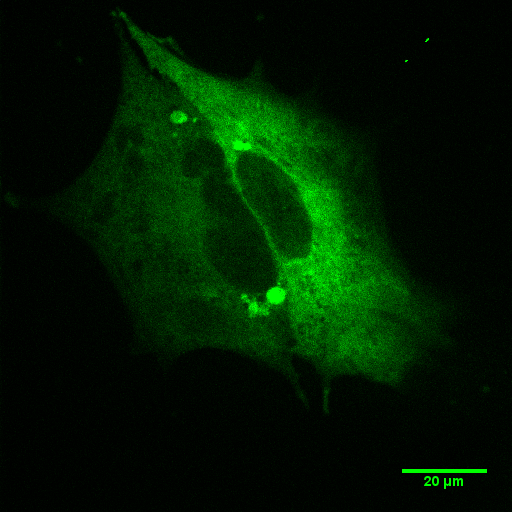
\includegraphics[width=3.5cm]{Figures/Exemple_C_GFP.png} 
 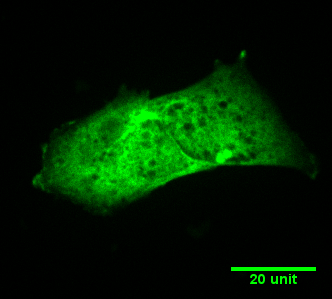
\includegraphics[width=3.5cm]{Figures/Exemple_H_GFP.png} 
 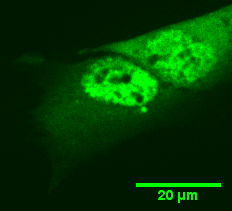
\includegraphics[width=3.5cm]{Figures/Exemple_N_2_GFP.png} 
 \caption{Exemples de cellules classées comme MRTF-A Cytoplasmique, Homogène et Nucléaire, de gauche à droite respectivement. En bleu, la phalloïdine marquant les filaments d'actine, en jaune la MRTF-A GFP.\label{Exemples_CHN}}

 \end{figure}
 
 \paragraph{Définition des évènements de changement d'état}
 
 Il peut arriver que les cellules classées comme il est décrit dans le paragraphe précédent changent de groupe au cours du temps. 
 Lorsqu'une cellule est suivie au cours du temps, on peut alors avoir des cellules qui passent d'un état à un autre, parfois plusieurs fois. 
 Pour chaque expérience on peut donc mesurer le nombre de cellules qui changent au moins une fois d'état, compter le nombre de changements ayant eu lieu (nombre strictement supérieur au précédent) et les classer en fonction de leur état de départ et d'arrivée. 
 Trois changements sont catégorisés comme \og entrants \fg : C $\rightarrow$ H, C $\rightarrow$ N et H $\rightarrow$ N. 
 Les trois autres sont catégorisés comme \og sortants \fg  : H $\rightarrow$ C, N $\rightarrow$ H et N $\rightarrow$ C. 
 
 
 \paragraph{Quantification}
 Dans un second temps, pour caractériser la répartition de MRTF-A dans la cellule, les intensités de fluorescence dans le cytoplasme, dans le noyau et dans une zone péri-nucléaire ont été mesurées et comparées. Cette méthode est plus précise mais allonge considérablement la durée du dépouillement. 
 Lorsque les images sont prises avec l'objectif 20X, nous ne prenons qu'un seul plan focal, mais il intègre le signal sur une certaine épaisseur de la cellule. Une zone épaisse, comme le noyau et la zone immédiatement autour, apparaîtra plus lumineuse en fluorescence qu'une zone fine comme un lamellipode, alors que la concentration en protéines est identique. 
 Pour comparer la concentration nucléaire à la concentration cytoplasmique, on remplace alors la mesure sur l'ensemble du cytoplasme par une mesure sur une zone autour du noyau qui a une épaisseur proche de celle du noyau. On compare alors l'intensité moyenne par pixel de chacune des deux zones.
 On peut également comparer la totalité du signal dans le noyau à sa totalité dans le cytoplasme, car le rapport taille du noyau sur taille de la cellule est relativement bien conservé d'une cellule à l'autre. 
 


\subsection{Influence des moyens d'observation sur l'équilibre entre MRTF-A et l'actine G}

Les C2C12 ont été transfectées avec un plasmide contenant une copie du gène MRTF-A humain adjoint d'une séquence eGFP. 
Cela nous permet en microscopie de fluorescence d'observer quelle proportion de MRTF-A GFP se trouve dans le noyau, et quelle proportion dans le cytoplasme de la cellule. 
En revanche, au total, MRTF-A est sur-exprimée dans la cellule, en proportions variables d'une cellule à l'autre. 
Si MRTF-A est sur-exprimée en trop grande quantité, il ne reste pas assez de G-actine dans la cellule pour la maintenir dans le cytoplasme, et elle peut alors s'accumuler dans le noyau. 
Nous avons donc essayé de transfecter la quantité minimale de protéine nécessaire pour mener à bien les observations. 

On peut observer sur des cellules fixées et marquées avec l'anti-corps MRTF-A endogène qu'à l'état naturel, MRTF-A est toujours dans le cytoplasme de la cellule. 
Lorsque nous observons la MRTF-A GFP, ce n'est pas toujours le cas, et une proportion plus ou moins grande, selon la quantité de plasmide qui a pénétré les cellules, est contenue dans le noyau.


L'objectif étant d'observer également le cytosquelette d'actine, nous avons mené des expériences avec un plasmide Actine mCherry, un plasmide LifeAct RFPn un plasmide F-tractine, des marquages DNaseI et phalloïdine sur cellules fixées, et enfin avec de la SiR-actine, successivement.
 
L'ajout d'actine mCherry augmente le réservoir d'actine monomérique de la cellule, et d'autant plus que l'actine fluorescente polymérise un peu moins bien que l'actine sauvage, et donc participe à maintenir MRTF-A dans le cytoplasme. 
Cette méthode d'observation est donc loin d'être neutre pour notre système, comme on le verra plus loin.
 
La LifeAct \parencite{riedl_lifeact:_2008} est une petite protéine qui se lie aux filaments d'actine, et qui n'est pas censée interférer avec la polymérisation des filaments. Cependant, nous avons constaté une tendance à la stabilisation des filaments avec la LifeAct. De plus, sa fluorescence était trop intense et interférait de manière importante avec le signal de MRTF-A GFP. 

La F-tractine \parencite{johnson_neuronal_2009} fonctionne de manière similaire, et donne des résultats similaires. 

La DNaseI et la phalloïdine nous permettent d'observer à la fois l'actine G et l'actine F dans la cellule, mais ne peuvent être utilisées que sur des échantillons fixés, ce qui limite fortement l'observation de la dynamique de réorganisation du cytosquelette.
 
Enfin, la SiR-actine \parencite{lukinavicius_fluorogenic_2014} est une molécule nouvelle dérivée de l'association du jasplakinolide et d'une rhodamine, qui peut être utilisée en faibles concentrations \emph{in vivo} pour observer les filaments d'actine. 


\section{Application d'une force locale avec les pinces magnétiques}

Pour réaliser des expériences sur les cellules transfectées MRTF-A GFP, il a fallu monter les pinces magnétiques sous le microscope confocal. 
L'observation se faisait avec un objectif 40X à air, dans la géométrie à courte distance, ce qui nous permet d'appliquer localement de grandes forces (plusieurs centaines de pN) mais nous empêche d'observer suffisamment bien la position de la bille pour faire des mesures rhéologiques. 
Dans un premier temps, l'objectif était simplement de voir si l'application d'une force par les pinces magnétiques était suffisante pour déclencher une relocalisation de MRTF-A dans les cellules musculaires. 

Une force constante d'environ 1nN a été appliquée sur les billes pendant 125 secondes, puis pendant les 125 secondes suivantes, la force est relâchée. Cette séquence est répétée 6 fois pendant un total de 1500 secondes (25 minutes). 

Nous avons réalisé ces expériences sur trois séries de C2C12 : transfectées avec MRTF-A GFP seule (37 cellules observées), tranfectées avec MRTF-A GFP et une Actine mCherry (16 cellules observées), et transfectées avec MRTF-A GFP et le LifeAct RFP, qui marque les filaments d'actine dans les cellules vivantes (42 cellules observées, dont 34 témoins). 
L'objectf de ces doubles transfections était d'observer en même temps que la localisation de MRTF-A la réorganisation du cytosquelette d'actine. 

Parmi ces expériences, certaines cellules ont été observées alors qu'elles n'avaient pas de bille attachée à leur cytosquelette : ce sont des cellules témoins, sur lesquelles le champ magnétique a été appliqué comme pour les autres, mais sur lesquelles le champ n'est pas censé avoir un effet quelconque. 

\begin{figure}
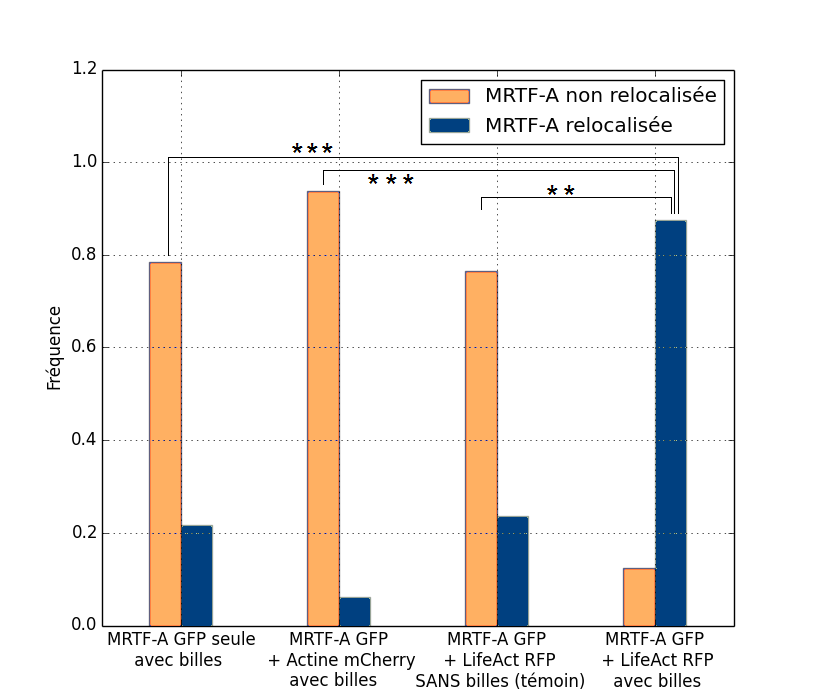
\includegraphics[scale=0.4]{Figures/Pinces_MRTFA_stars_colors.png} 
\caption{Proportion des cellules observées pour lesquelles MRTF-A GFP change (en vert) ou ne change pas (en bleu) de localisation dans la cellule au cours de l'expérience. * : $p<\frac{0.05}{4}$ , ** $p<\frac{0.01}{4}$, *** $p<\frac{0.001}{4}$ (réalisés avec un test de Fisher et une correction pour les comparaisons multiples)\label{MRTF-A Pinces}}
\end{figure}

On peut voir sur la figure \ref{MRTF-A Pinces} que l'ajout d'actine exogène réduit le nombre de cellules pour lesquelles MRTF-A change de localisation, mais de manière non significative  \footnote{ Il est à noter que vu le petit nombre de cellules observées, ces différences non significatives pourraient le devenir si l'on observait plus de cellules. }, alors que l'ajout de Life Act RFP a l'effet inverse de manière significative.
En effet, en ajoutant de l'actine mCherry, on augmente la quantité totale de G-actine dans la cellule, et ce d'autant plus que l'actine fluorescente polymérise un peu moins bien que l'actine sauvage. Comme plus de G-actine est disponible pour se lier à MRTF-A, celle-ci est d'autant plus susceptible d'être liée à l'actine et donc cytoplasmique. 
Si la réserve d'actine monomérique est grande, une polymérisation d'actine en réponse à la force appliquée ne sera pas forcément suffisante pour dépléter la réserve de G-actine excédentaire.

Au contraire, la LifeAct, en se liant aux filaments d'actine, peut les stabiliser en conformation polymérisée. En stabilisant la F-actine, la LifeAct rend donc la cellule beaucoup plus sensible à un recrutement de G-actine pour former de nouveaux filaments, et MRTF-A est plus susceptible de se retrouver sans liaison avec l'actine, et donc nucléaire.

De plus, on peut voir en comparant avec les expériences LifeAct témoin sans bille que l'application d'une force sur la cellule a un effet significatif sur la relocalisation de MRTF-A. 

On peut également remarquer que les résultats pour MRTF-A GFP seule sont identiques aux résultats avec LifeAct RFP mais sans application de force. 
On peut raisonnablement supposer que la force appliquée n'est pas suffisante ou n'est pas appliquée suffisamment longtemps pour réorganiser significativement le cytosquelette lors des expériences MRTF-A GFP seule, ce qui explique que leur activité soit proche de celle des cellules témoins. 
La présence de Life-Act RFP stabilisant les filaments, la réserve d'actine monomérique est plus faible dans les cellules doublement transfectées MRTF-A GFP + LifeAct RFP, ce qui les rend plus sensibles : une contrainte plus faible suffit à dépléter suffisamment la réserve de G-actine. 

\begin{figure}
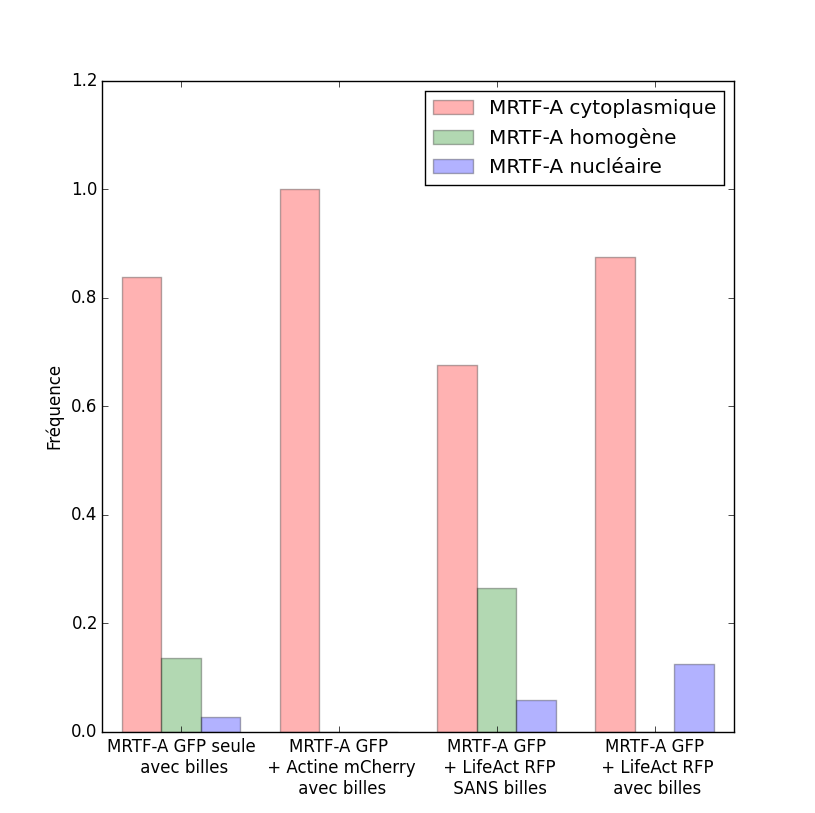
\includegraphics[scale=0.4]{Figures/CHN_pinces.png} 
\caption{Répartition de MRTF-A dans les cellules avant application de la force. \label{CHN_pinces}}
\end{figure}

On peut remarquer que la répartition initiale de localisation de MRTF-A entre les différentes expériences est relativement semblable, ce qui implique que le changement d'activité observé sur la figure \ref{MRTF-A Pinces} n'est pas dû à l'état initial de MRTF-A dans ces cellules. 
Cependant, on peut noter une augmentation de la quantité de cellules avec MRTF-A cytoplasmique avec l'actine mCherry, ce qui est cohérent avec la surexpression de l'actine. Cette augmentation n'est pas significative, probablement en raison d'un nombre de cellules observées insuffisant. On note à l'inverse une augmentation de la quantité de MRTF-A nucléaire avec la LifeAct, ce qui est également cohérent avec l'hypothèse d'une stabilisation des filaments par la LifeAct. 

\section{Application d'une déformation globale avec l'étireur : \'Etude qualitative et dynamique}

Les pinces magnétiques, lorsqu'il s'agit de suivre la dynamique sur une durée de quelques dizaines de minutes, ont l'inconvénient majeur de ne pouvoir opérer que sur une cellule à la fois. Comme les comportements observés sur les cellules sont extrêmement divers, il faut alors beaucoup de temps pour obtenir une population de cellules de taille acceptable avec cette méthode. 

C'est pourquoi les expériences sur MRTF-A ont été poursuivies par des déformations à l'aide d'un substrat étirable. De cette manière, on peut observer en général une trentaine de cellules pendant deux heures, là où précédemment on n'aurait pu observer que 4 cellules, chacune pendant 30 minutes. 



\subsection{\'Etat de référence}

Avant de comparer ce qu'il se passe pour différents taux d'étirement, il est nécessaire de mesurer quel est l'état de référence de notre système, qui sera le témoin. 

L'état de référence est construit à partir de cellules qui ont été transfectées en MRTF-A GFP seulement, puis ensemencées et montées comme si elles allaient être étirées. 
Aucun rinçage n'a été effectué avant expérience pour éliminer l'effet du changement de milieu de culture (la section \ref{Rinçage} aborde ce sujet en détail). 

La dynamique de référence des cellules a été observée pendant deux heures de manière strictement identique à une expérience où l'étirement est non-nul, afin de pouvoir quantifier la fréquence naturelle des changements de localisation de MRTF-A pendant cette durée. 

\begin{figure}
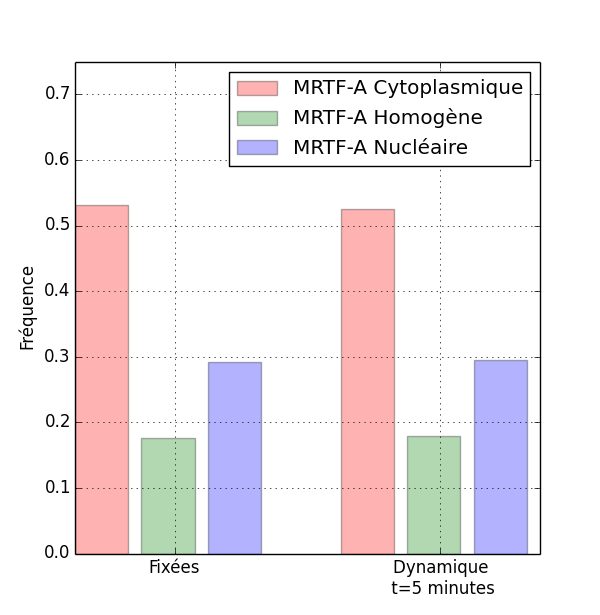
\includegraphics[scale=0.5]{Figures/Reference.png} 
\caption{Répartition entre les trois états pour des cellules fixées immédiatement après un montage sans rinçage et sans étirement (n=7, 963 cellules) et lors de l'observation en direct après 5 minutes d'observation sans étirement (n=5, 41 cellules). La différence n'est pas significative (p=0.995, G-test).
\label{Référence}}
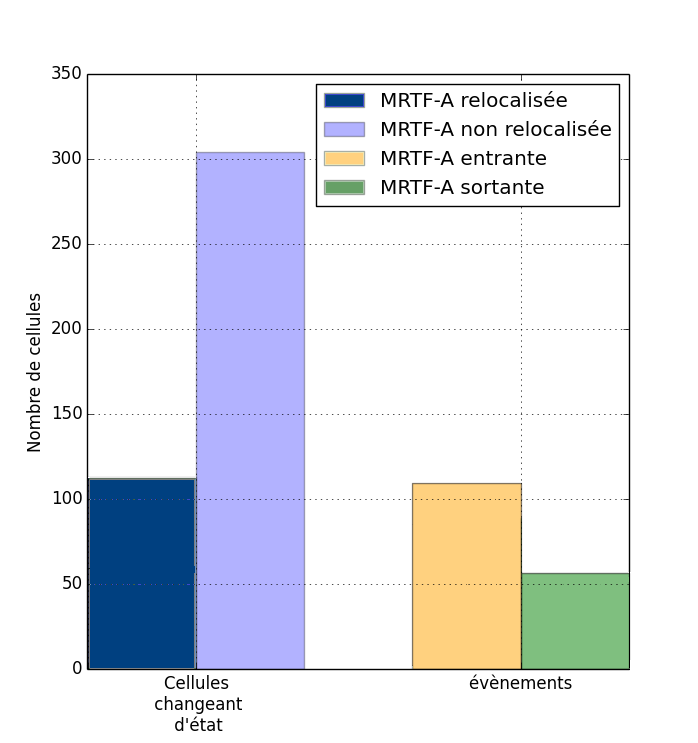
\includegraphics[scale=0.4]{Figures/Reference_transloc.png} 
\caption{Quantité de cellules changeant au moins une fois d'état pendant 2 heures d'observation et direction de ces changements \label{Ref_transloc}}
\end{figure}

\begin{figure}
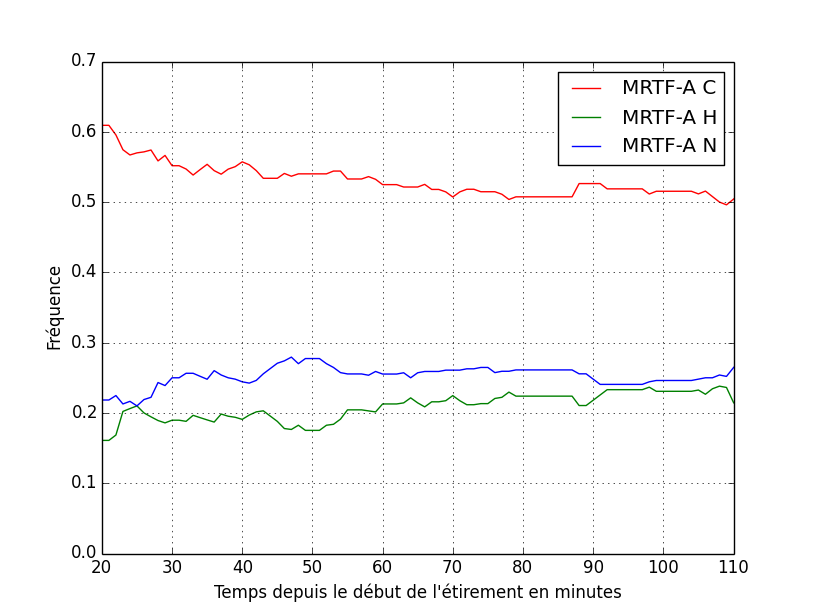
\includegraphics[scale=0.4]{Figures/CHN_vs_Temps_reference.png} 
\caption{\label{Reference_dynamique} \'E{}volution de la proportion de cellules ayant MRTF-A dans chacune des trois localisations au cours du temps lors d'une expérience témoin où l'on a monté à l'avance la lamelle dans l'étireur et où l'on n'applique aucune contrainte.}
\end{figure}

On peut observer la répartition entre les trois états est la même lors des expériences fixées immédiatement après montage et après 5 minutes d'étirement sur la figure \ref{Référence}.
Cela peut indiquer qu'il n'y a aucune réponse de la part des cellules durant les 5 premières minutes, mais cela n'exclut pas une réaction très rapide qui reviendrait à l'équilibre pendant ce laps de temps, même si ceci semble peu probable. 

Le lecteur attentif aura remarqué que cette répartition est différente de celle présentée en figure \ref{MRTF-A Pinces}. 
Cela est dû aux différences dans la préparation des cellules dans les deux expériences, car la transfection n'était pas faite dans les conditions optimales lors des expériences de pinces magnétiques. 
La quantité de plasmide ayant pénétré dans les cellules était plus faible, et la quantité de cellules ayant MRTF-A dans le noyau (Homogène ou Nucléaire) l'est également. 


L'évolution de l'état de base au cours du temps est présentée sur la figure \ref{Reference_dynamique}. On peut observer que la proportions des différents états reste relativement stable, avec une légère diminution de la quantité de MRTF-A Cytoplasmique au cours du temps. 
Pendant la durée totale de l'expérience, on peut observer sur la figure \ref{Ref_transloc} qu'environ 27\% des cellules ont changé d'état au moins une fois, et que dans les deux tiers des cas, ces changements se font vers des états où MRTF-A est plus nucléaire qu'avant (évènements \og entrants \fg). 


\subsection{Effet de la sur-expression d'actine mCherry}

Lors de la double transfection MRTF-A GFP et Actine mCherry, nous avons accès à deux populations de cellules simultanément. En effet, certaines cellules expriment les deux plasmides, tandis que d'autres n'expriment que MRTF-A GFP, et peuvent donc servir de témoin de l'effet de l'Actine mCherry. 
Ces expériences ont été étirées à 10 ou 30\%, les résultats présentés ici sont les populations après 20 minutes d'étirement. Pendant les deux heures d'observation, la répartition des cellules est restée stable, et la fréquence des changements d'état est égale à celle observée pour les cellules témoins. 

De manière similaire à ce qui était observé figure \ref{MRTF-A Pinces} pour les expériences de pinces magnétiques, la sur-expression d'actine causée par l'introduction d'un plamide d'actine mCherry cause des changements importants et significatifs à la localisation de MRTF-A dans la cellule. 

Parmi les cellules qui expriment l'actine mCherry, la proportion de celles ayant MRTF-A dans le cytoplasme augmente, aux dépens des cellules ayant MRTF-A dans le noyau, car il y au total plus de G-actine disponible dans la cellule pour empêcher MRTF-A d'être importé dans le noyau. 

\begin{figure}
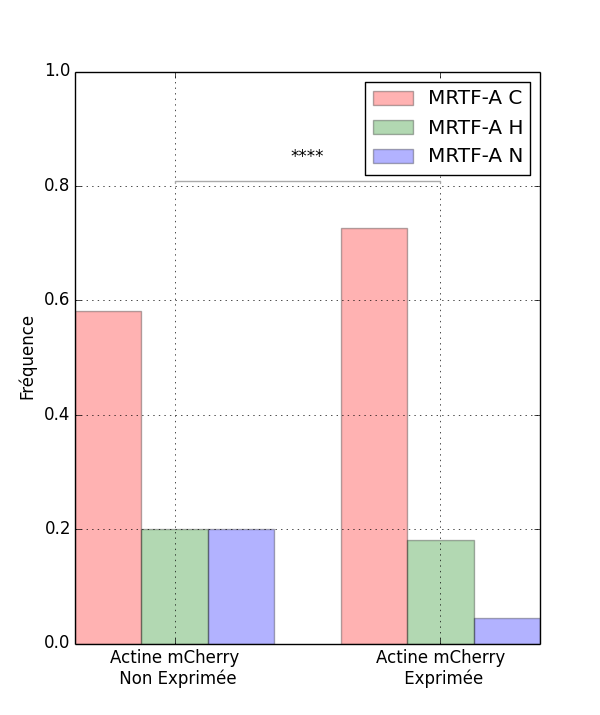
\includegraphics[scale=0.4]{Figures/AMC.png}
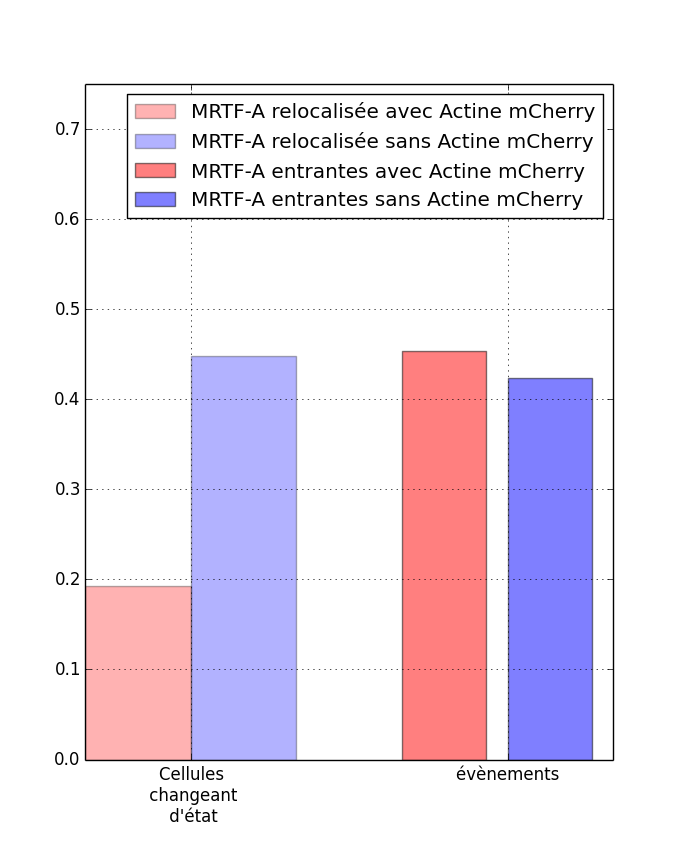
\includegraphics[scale=0.3]{Figures/AMC_translob.png}
\caption{\label{AMC}Répartition initiale pour des cellules issues des mêmes expériences exprimant ou non le plasmide Actine mCherry (683 cellules témoin et 538 cellules expriment l'Actine mCherry). **** : $p<10^{-4}$}\caption{\label{AMC_transloc}Proportion de cellules changeant au moins une fois d'état et proportion d'entrantes et de sortantes, pour les même expériences, selon que l'Actine mCherrry est exprimée ou non.}
\end{figure}

Lorsque l'on compare le nombre de cellules ayant changé d'état au moins une fois pendant les deux heures d'observation, on voitt qu'il est divisé par deux lorsque l'actine mCherry est exprimée par les cellules, mais cela ne change pas la répartition des évènements entre entrants ou sortants. 
Pourtant, on aurait pu s'attendre à ce qu'il y ait plus d'évènements entrants que de sortants dans la mesure ou il y a nettement plus de cellules où MRTF-A est cytoplasmique et donc ne peut faire qu'entrer dans le noyau. 

Finalement, la sur-expression d'actine mCherry bloque le changement de localisation de MRTF-A par rapport à des cellules dans les même conditions n'exprimant pas le plasmide, ce qui est facilement expliqué par le fait qu'une plus grande réserve d'actine monomérique va séquestrer MRTF-A dans le cytoplasme de manière plus efficace.

\subsection{Effet du rinçage et du montage préalables \label{Rinçage}}

En faisant des expériences témoin durant lesquelles aucun étirement n'était imposé, nous avons commencé à soupçonner qu'une ou plusieurs étapes de la préparation de l'échantillon pouvaient interférer avec les expériences. 
Deux étapes ont été testées : la première est l'étape durant laquelle on sort la lamelle de la plaque six puits pour la monter dans l'étireur, et qui implique des contraintes mécaniques sur la lamelle ; la seconde est l'étape de rinçage durant laquelle le milieu de culture des puits était remplacé par du milieu neuf dans l'étireur, ce qui pouvait induire une variation de la concentration en sérum. 

Pour l'étape de montage, nous avons testé le montage juste avant l'expérience (Montées), et le montage la veille au soir (Prémontées). 
Le rinçage est toujours effectué en même temps que le montage. 


\begin{figure}
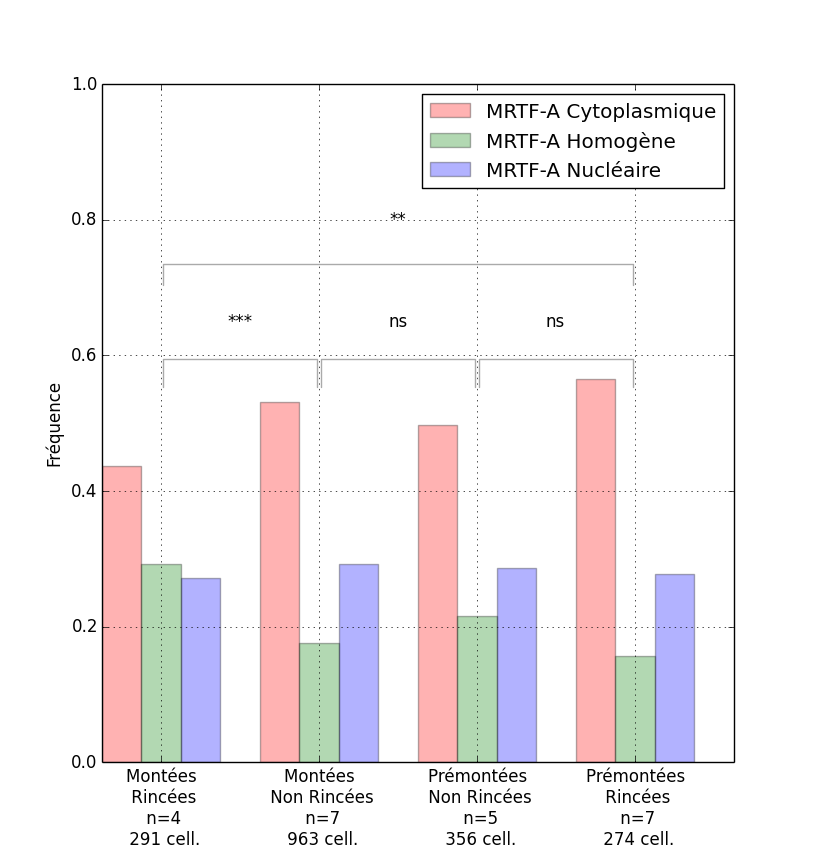
\includegraphics[scale=0.5]{Figures/CHN_montage_rincage.png} 
\caption{\label{CHN_montage} Influence sur la localisation de MRTF-A des contraintes mécaniques dues au montage de la lamelle dans l'étireur (Montage) et de la variation de concentration en sérum due au remplacement du milieu de culture par du milieu neuf au moment du montage (Rinçage). Montées : montage à $t-5$ minutes, Prémontées : montage à $t-18$ heures, rinçage au même moment.
Tous les tests on été réalisés avec un G-test d'indépendance t et une correction de Bonferroni pour les comparaisons multiples. ** : $p<\frac{0.01}{4}$ et *** : $p<\frac{0.001}{4}$}
\end{figure}

On peut voir sur la figure \ref{CHN_montage} que lorsque les cellules sont rincées juste avant l'expérience (Montées Rincées vs Montées Non Rincées), il y a significativement moins de cellules pour lesquelles MRTF-A est majoritairement cytoplasmique. 
Comme son nom l'indique, Serum Response Factor est puissamment activé par le sérum, et ici le seul rinçage avec du milieu neuf suffit à activer la voie de signalisation MRTF-A/SRF et changer la localisation de MRTF-A d'une partie des cellules. 
On également constater que lorsque le rinçage est effectué la veille (Prémontées Rincées vs Prémontées Non Rincées), il n'y a plus aucun effet. 

On peut finalement voir que l'étape du montage n'a pas la même influence selon qu'il y a rinçage ou non. Sans rinçage, cette étape n'a pas d'influence significative sur l'état des cellules, en revanche avec rinçage, on peut remarquer que le montage a tendance à augmenter la quantité de cellules ayant MRTF-A dans le cytoplasme aux dépens de celles l'ayant réparti de manière homogène. 

Une fois ces résultats mis en évidence, nous avons réalisé la suite des expériences en évitant scrupuleusement de changer le milieu de culture dans lequel baignent les cellules le jour même de l'expérience. 

\subsection{Résultats pour l'étirement 10\%}

Dans les mêmes conditions que pour le témoin, c'est-à-dire avec des lamelles montées la veille des expériences en conservant le même milieu de culture, et sans plasmide Actine mCherry, nous avons appliqué un étirement de 10\% au temps t=0, puis observé les cellules toutes les 10 minutes pendant 120 minutes en maintenant l'étirement. 

La figure \ref{CHN_dyn_Et10} montre la fréquence dans la population de cellules de chacune des trois localisations possibles de MRTF-A GFP à l'intérieur de la cellule en fonction du temps écoulé depuis le début de l'étirement. 
 
Dès le début de l'observation \footnote{Les vingt premières minutes après l'étirement sont consacrées à la recherche de cellules exprimant la MRTF-A GFP. C'est pourquoi le début de l'observation est placé au moment où la population de cellules repérées a atteint un nombre suffisant, typiquement une trentaine de cellules.}, la proportion de cellules ayant MRTF-A dans le cytoplasme est inférieure à celle du témoin : 60 \% de cellules avec MRTF-A cytoplasmique pour le témoin contre moins de 50\% pour les cellules étirées. Cet écart se creuse avec le temps, jusqu'à la fin de la période d'observation, deux heures après le début de l'étirement, où il reste encore 50 \% de cellules avec MRTF-A cytoplasmiques dans le cas témoin, mais environ 35 \% lorsque les cellules ont été étirées. 

Au contraire, les cellules ayant MRTF-A répartie de manière homogène sont plus nombreuses : plus de 25 \% de cellules avec MRTF-A répartie de manière homogène après 20 minutes d'étirement contre moins de 20  \% pour le témoin. 
Si initialement la quantité de cellules ayant MRTF-A clairement accumulée dans le noyau est identique dans les deux expériences, à partir d'une heure d'étirement, on observe une croissance de cette population chez les cellules étirées par rapport aux témoins. Au bout de 100 minutes d'étirement, les cellules ayant MRTF-A dans le noyau sont un peu plus de 20 \% dans la population témoin, mais 35\% dans la population étirée. 



\begin{figure}
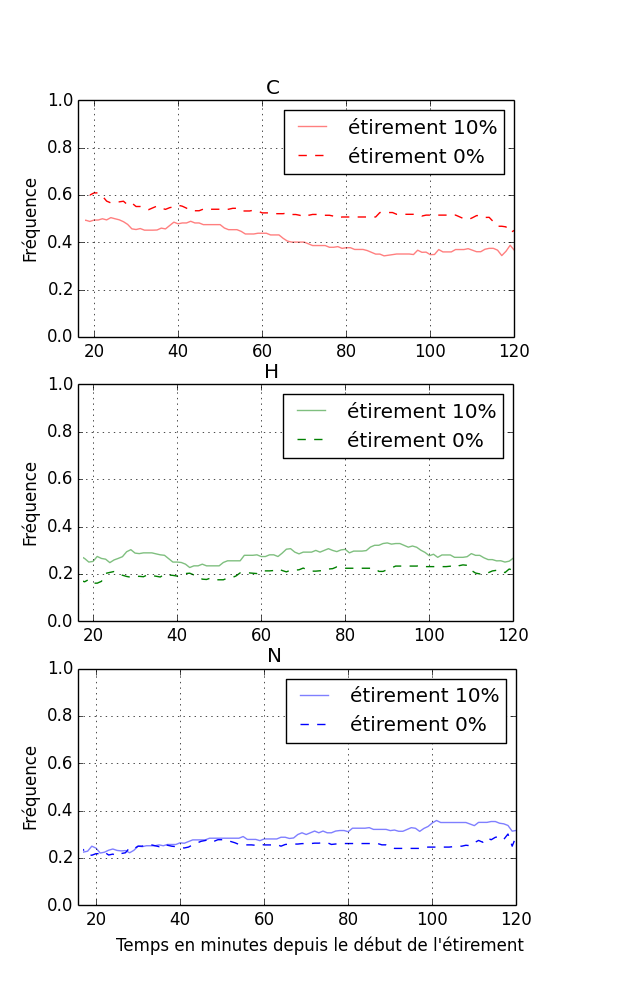
\includegraphics[scale=0.4]{Figures/Etirement10_vs_0_dynamique.png} 
\caption{\label{CHN_dyn_Et10} Comparaison de l'évolution de la fréquence de chaque localisation de MRTF-A au cours du temps après 10\% d'étirement et dans les expériences témoin (n=5 et 141 cellules dans les deux cas)}
\end{figure}

La figure \ref{transloc_dyn_Et10} présente de manière plus détaillée tous les évènements de changement de localisation de MRTF-A GFP observés pendant l'expérience. 
Comme chaque cellule n'est observée qu'une fois toutes les dix minutes, il existe une incertitude temporelle sur le moment auquel a eu lieu la transition entre un état et un autre. C'est pourquoi, pour représenter les évènements au cours du temps, le nombre d'évènements a été compté pendant un intervalle [t-5 minutes ; t+5 minutes], puis il a été normalisé en le divisant par le nombre de cellules qui sont observées durant cet intervalle. 
Chacun des six graphes représente l'occurrence d'un évènement différent au cours du temps, pour l'expérience d'étirement et son témoin. 

On voit sur la figure \ref{transloc_dyn_Et10} une vague importante d'évènements C$\rightarrow$ H et H $\rightarrow$ N (donc entrants) se produire lors de l'étirement 10\%. Les évènements sortants restent quant à eux au même niveau pendant l'expérience d'étirement et pendant le témoin. 

Sur la figure \ref{CHN_dyn_Et10}, on avait pu remarquer que la population de cellules avec MRTF-A nucléaire ne croissait par rapport à l'expérience témoin qu'à partir de 60 minutes après étirement. On peut voir le même effet sur le graphe \ref{transloc_dyn_Et10}, où l'augmentation visible des transitions H $\rightarrow$ N ne commence qu'à partir de 60 minutes après étirement. 
En effet, la première vague d'évènements H $\rightarrow$ N est issue de cellules où MRTF-A était homogène depuis le début de l'expérience. La seconde vague, visible entre 60 et 80 minutes, est composée pour moitié de cellules qui avaient MRTF-A dans le cytoplasme au début de l'expérience, puis qui sont passées de l'état C à H pendant la première heure après étirement, et continuent à accumuler MRTF-A dans le noyau pendant l'heure suivante. 

Les évènements rapides, C $\rightarrow$ N et N $\rightarrow$ C sont très rares : trois évènements entrants sont observés au total, un lors de l'expérience témoin et deux lors de l'étirement, alors qu'aucun évènement sortant n'a été observé. 

La figure \ref{activite_Et10} représente le nombre d'évènements entrants et sortants par cellule pour l'expérience d'étirement et son témoin. 
On peut observer que le nombre d'évènements sortants ne varie pas avec l'étirement alors que le nombre d'évènements entrants est multiplié par trois. Cela reflète bien ce qui était déjà visible sur la figure \ref{transloc_dyn_Et10}. 

\begin{figure}
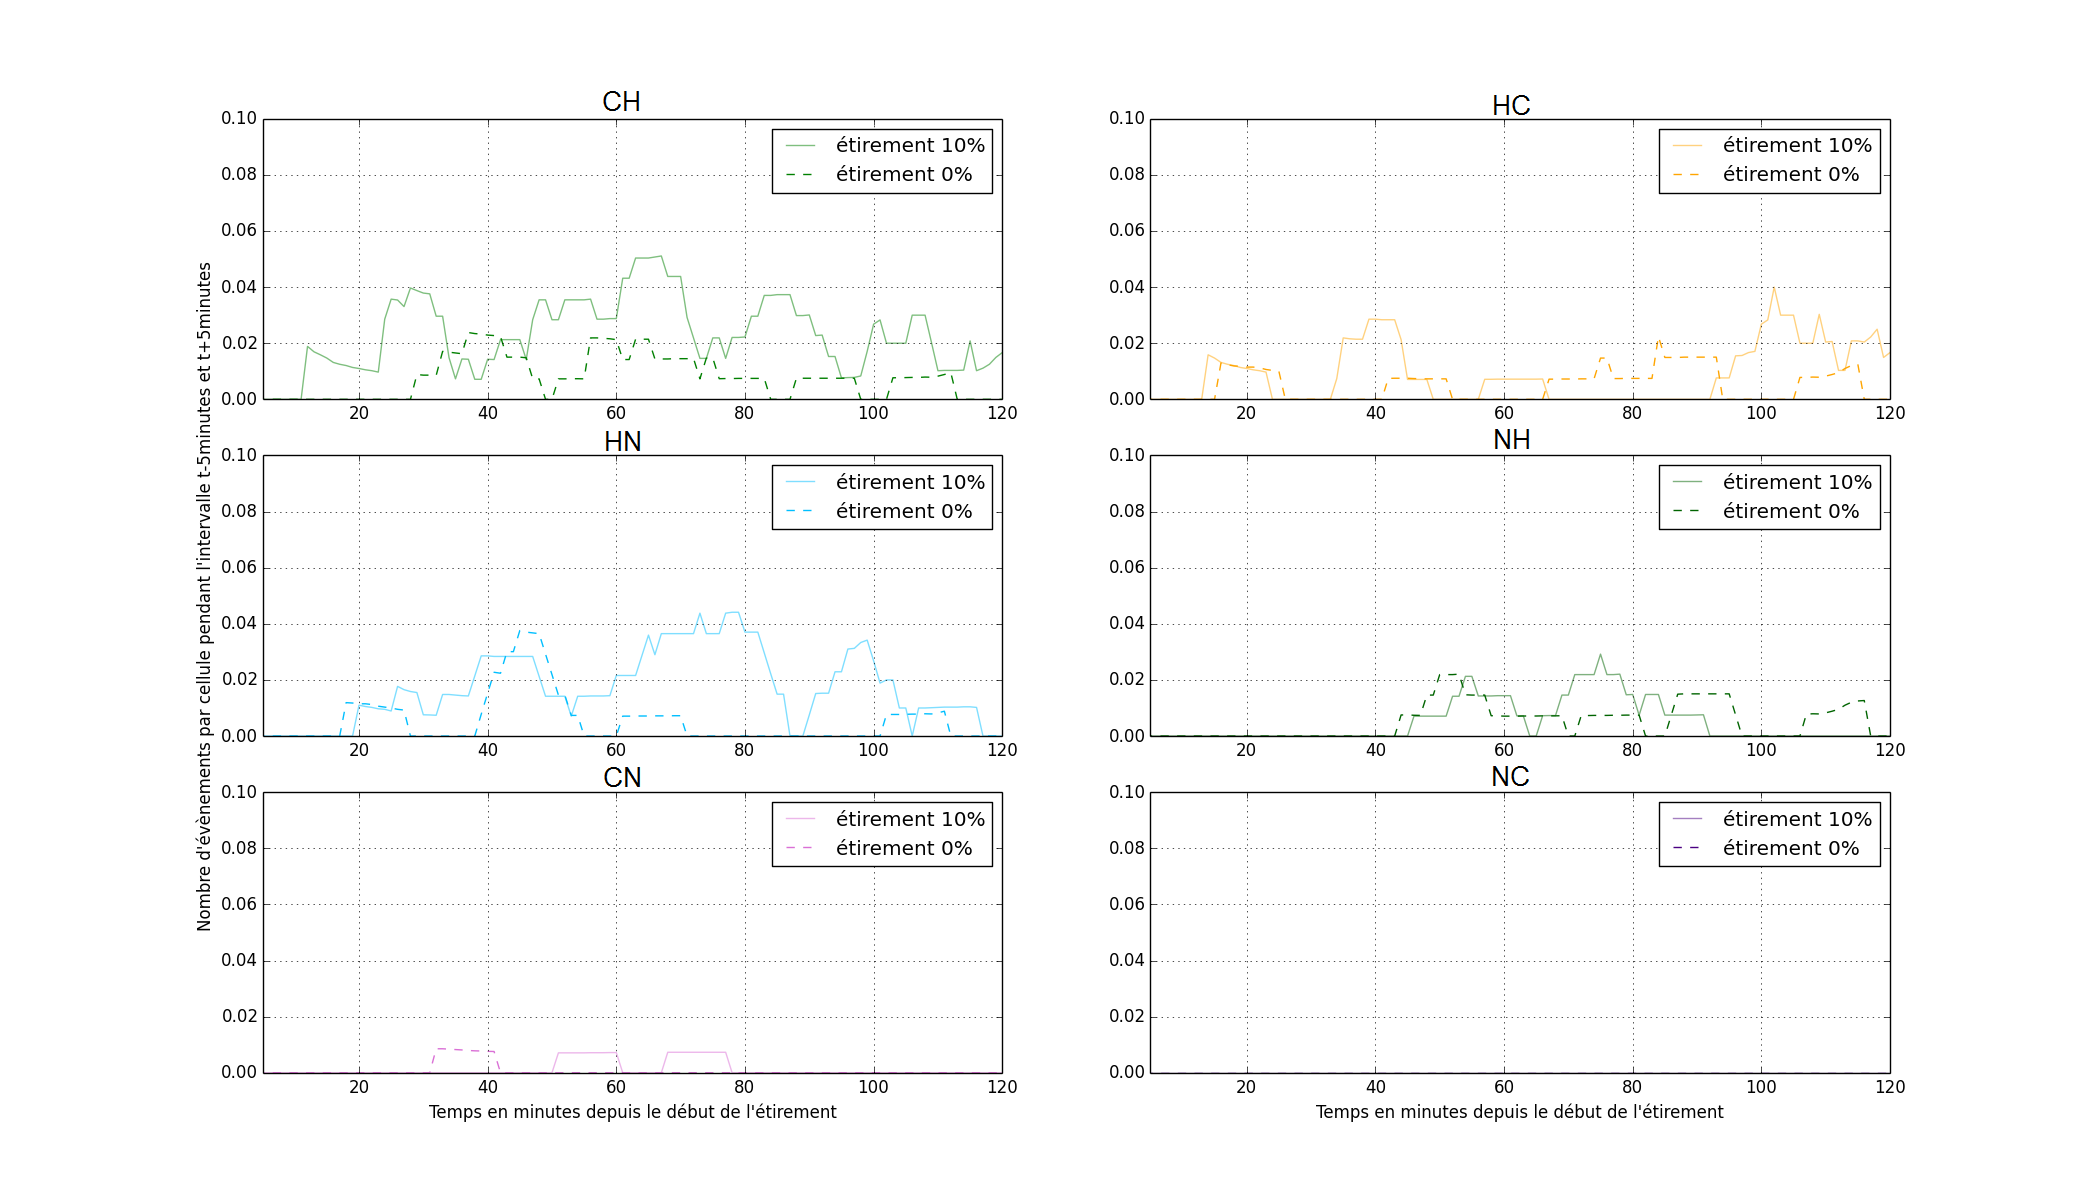
\includegraphics[scale=0.33]{Figures/Etirement10_vs_0_translocations.png} 
\caption{\label{transloc_dyn_Et10} Nombre d'évènements ayant eu lieu pendant la fenêtre [t-5min,t+5min] pour chaque type de transition possible divisé par le nombre de cellules observées. La première lettre du titre de chaque graphe représente l'état initial de la localisation de MRTF-A dans la cellule, la seconde lettre l'état final. Par exemple le premier graphe "CH" représente le nombre de cellules dans lesquelles MRTF-A est passée d'une localisation cytoplasmique à homogène dans l'intervalle [t-5min;t+5min] divisé par le nombre total de cellules.}
\end{figure}

\begin{figure}
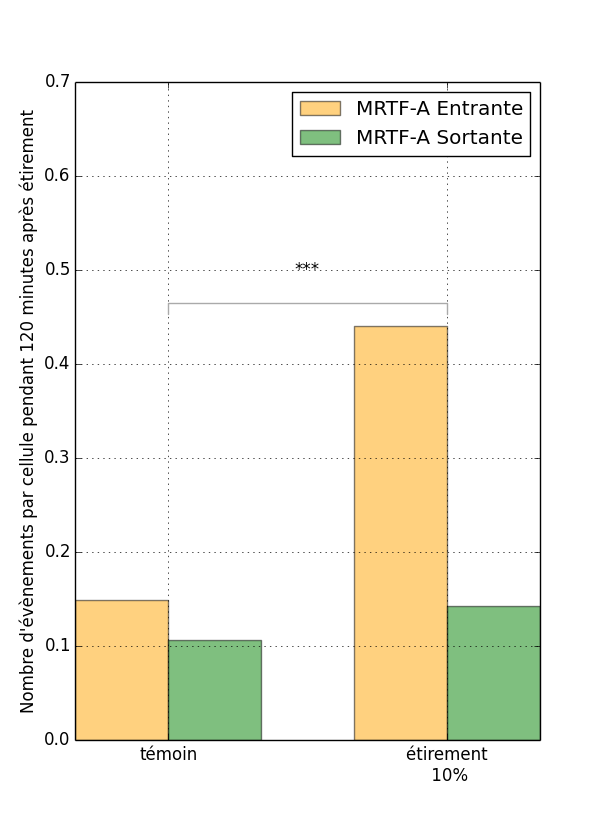
\includegraphics[scale=0.4]{Figures/Etirement10_vs_temoin_activite.png} 
\caption{\label{activite_Et10} Nombre d'évènements entrants ou sortants par cellule observée pendant 120 minutes, pour l'étirement 10\% et pour le témoin. p=0.0003 }
\end{figure}

On peut donc en conclure que l'étirement est corrélé à une augmentation de la relocalisation de MRTF-A du cytoplasme vers le noyau, de manière à peu près continue pendant les deux heures d'étirement et d'observation. 

De manière générale, les résultats sont conformes à ce qui était attendu : l'application d'une contrainte mécanique sur les cellules entraîne l'accumulation lente et progressive de MRTF-A dans le noyau. 

La première hypothèse pour expliquer cette accumulation nucléaire de MRTF-A est que la contrainte oblige les cellules à renforcer leur cytosquelette d'actine, et donc crée un manque de monomères d'actine.  

Le suivi dynamique nous montre qu'il y a peu de changements qui se produisent pendant les vingt premières minutes d'étirement. Par la suite, l'augmentation de la quantité d'évènements entrants est maintenue pendant les deux heures que dure l'observation. 


\subsection{Résultats pour l'étirement 30\%}

Initialement, on s'attendait à voir pour l'étirement le plus fort les mêmes effets que pour l'étirement 10\%, mais plus importants. 
Ce n'est pas du tout ce qui est ressorti des expériences, qui ont montré à peu près le contraire. 

En effet, si l'on observe l'évolution des trois populations différentes par rapport au témoin, on peut voir sur la figure \ref{Et30_CHN} que la quantité de cellules avec MRTF-A majoritairement cytoplasmique augmente, passant d'environ 50 \% à t=20 minutes à plus de 60\% au bout de 80 minutes d'étirement, lorsqu'elle atteint son maximum. 
Au contaire, on peut voir à t=80 minutes que les cellules pour lesquelles MRTF-A GFP est homogène, qui comptaient pour un quart de la population initialement, ne représentent plus que 15 \% du total. 
Les cellules ayant MRTF-A majoritairement nucléaire sont elles en proportion inférieure à 20 \% pendant toute la durée de l'expérience. 

On constate donc que l'évolution de la population est à l'inverse de celle observée pour un étirement plus faible : de plus en plus de MRTF-A est confiné dans le cytoplasme. 

\begin{figure}
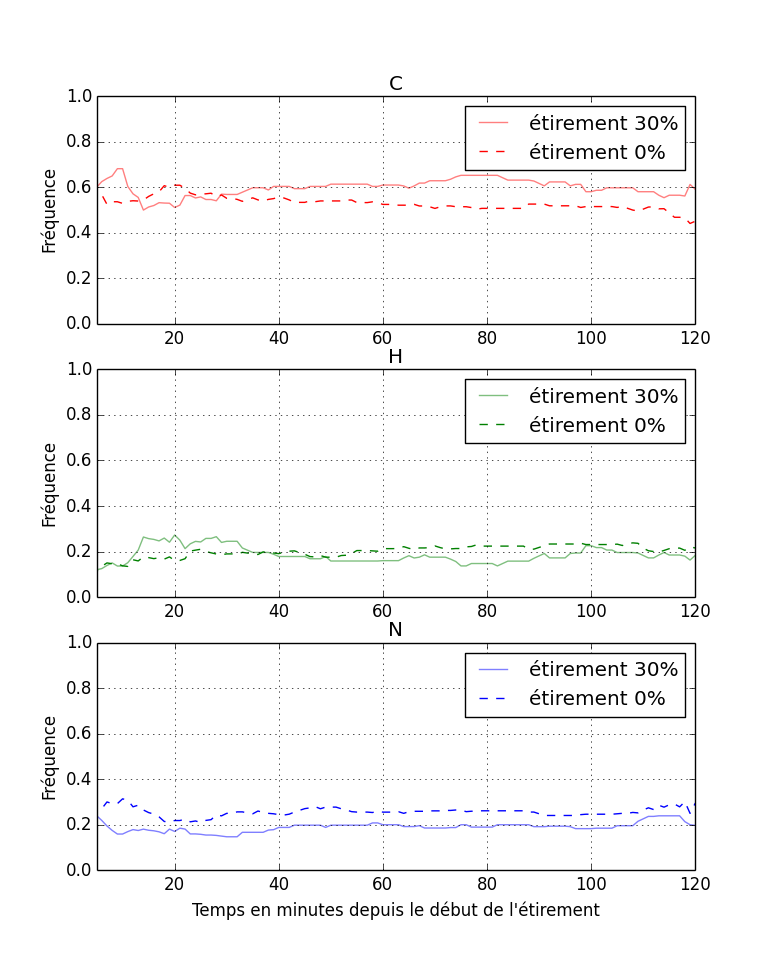
\includegraphics[scale=0.5]{Figures/Etirement30_vs_0_dynamique.png} 
\caption{\label{Et30_CHN} Comparaison de l'évolution de la fréquence de chaque localisation de MRTF-A au cours du temps après 30\% d'étirement ou dans les expériences témoin (n=5 et 141 cellules pour le témoin, n=3 et 102 cellules pour l'étirement 30\%)}
\end{figure}

De plus, sur la figure \ref{Et30_transloc}, on peut constater qu'il y a dès le début de l'expérience un pic net dans le nombre d'évènements sortants H $\rightarrow$ C entre 20 et 40 minutes, pendant lequel les évènements sont 6 fois plus nombreux que pour le témoin. Un pic synchronisé est visible dans les transitions sortantes N $\rightarrow$ H. 

Au contraire, les évènements entrants sont au même niveau que pendant l'expérience témoin pendant les 80 premières minutes de l'étirement 30\%. À partir de t=80 minutes, on observe que le comportement s'inverse : il y a un grand nombre d'évènements entrants et les évènements sortants redescendent au niveau du témoin. 

Un pic d'évènements sortants devrait être lié à une grande quantité de G-actine libérée dans ces cellules, de manière très rapide, ce qui nous amène naturellement à poser l'hypothèse d'une destruction brutale du cytosquelette en réponse à un déformation trop forte. Cette défaillance du cytosquelette d'actine à 30 \% de déformation est surprenamment cohérente avec les mesures faites sur de l'actine \textit{in vitro} \cite{janmey_mechanical_1994}. 
À partir de t=80 minutes, lorsque les évènements entrants commencent à augmenter, on verrait alors les conséquences d'une reconstruction progressive du cytosquelette. 

 
\begin{figure}
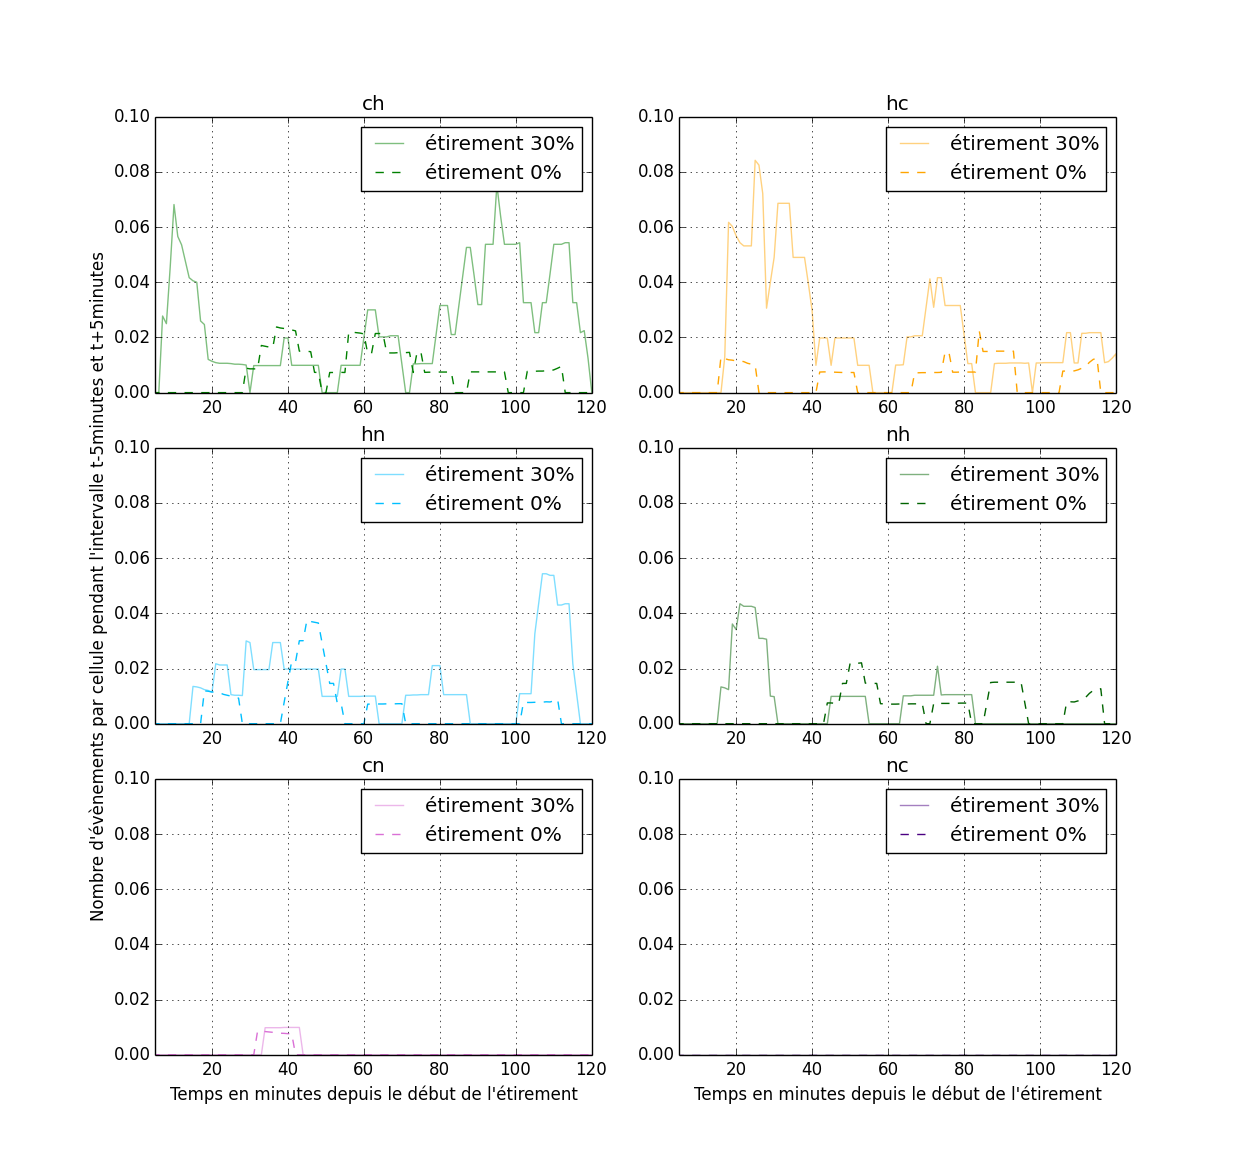
\includegraphics[scale=0.5]{Figures/Etirement30_vs_0_translocations.png}
\caption{\label{Et30_transloc} Nombre d'évènements ayant eu lieu pendant la fenêtre [t-5min,t+5min] pour chaque type de transition possible divisé par le nombre de cellules observées. La première lettre du titre de chaque graphe représente l'état initial de la localisation de MRTF-A dans la cellule, la seconde lettre l'état final. Par exemple le premier graphe "CH" représente le nombre de cellules dans lesquelles MRTF-A est passée d'une localisation cytoplasmique à homogène dans l'intervalle [t-5min;t+5min] divisé par le nombre total de cellules. }
\end{figure}

\begin{figure}
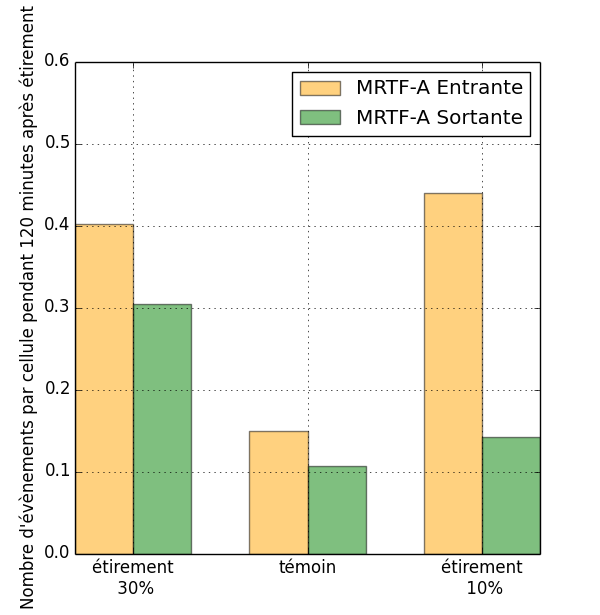
\includegraphics[scale=0.5]{Figures/Etirement30_vs_temoin_activite.png}
\caption{\label{Et30_activite} Quantité de changements d'état par cellule pour les trois conditions différentes (p=$10^{-4}$, G-test d'indépendance).}
\end{figure}

On peut finalement remarquer que comme lors de l'autre expérience d'étirement, une grande partie des cellules change au moins une fois d'état pendant les deux heures d'observation, comme on peut le voir sur la figure \ref{Et30_activite}, mais il y a nettement moins de déséquilibre entre les évènements entrants et sortants (p=0.014, figure \ref{Et30_ES}). 

 \begin{figure}
 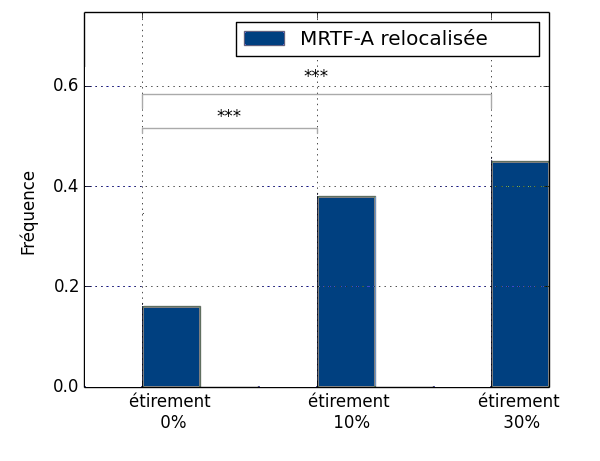
\includegraphics[scale=0.5]{Figures/Activite.png} 
 \caption{\label{Et30_ES} Comparaison pour les deux étirements et le témoin de la quantité de cellules qui changent d'état au moins une fois}
 \end{figure}
 
Initialement, on souhaitait regarder en parallèle l'état du cytosquelette d'actine et la localisation de MRTF-A. 
Malheureusement, comme on peut le voir tant en expériences de pinces magnétiques que d'étirement, l'expression d'actine mCherry et de LifeAct RFP perturbe de manière trop importante le cytosquelette d'actine pour être utilisée pendant les expériences. 
C'est pourquoi les expériences ont été faites avec MRTF-A GFP seulement, ce qui nous prive d'informations sur l'état du cytosquelette.
Afin de vérifier les hypothèses posées pour expliquer les observations aux deux étirements testés,deux approches ont été testées. La première est d'utiliser la SiRactine, un nouveau marqueur fluorescent pour les filaments d'actine, qui s'utilise directement sur les cellules sans rinçage. 
La seconde est de passer aux expériences fixées, qui ont l'avantage de pouvoir être marquées à la fois pour l'actine F et pour l'actine G. Pour cette dernière, il n'existe actuellement aucune sonde commerciale fonctionnant sur des cellules vivantes. 

\subsection{Visualisation de l'actine pendant l'étirement 10\%}

\subsubsection{Utiliation de F-tractine RFP}


La LifeAct a montré ses effets pendant les expériences sur les pinces magnétiques, elle n'a donc pas été réutilisée pour les expériences d'étirement. 

La F-tractine est un marqueur des filaments qui fonctionne de manière similaire, mais est réputé perturber moins le cytosquelette d'actine. Elle est constituée des 66 premiers acides aminés d'une protéine qui se lie aux filaments d'actine. Comme la LifeAct, son gène doit être transfecté préalablement dans la cellule. 

Malheureusement, les expériences qui suivent n'ont pas pu être réalisées exactement dans les mêmes conditions que les expériences précédemment décrites. En effet, suite au rachat de notre fournisseur, la nanofectine n'est plus commercialisée. Les transfections MRTF-A GFP des expériences avec la F-tractine et avec la SiRactine ont donc dû être réalisées avec de la lipofectamine. 

\begin{figure}
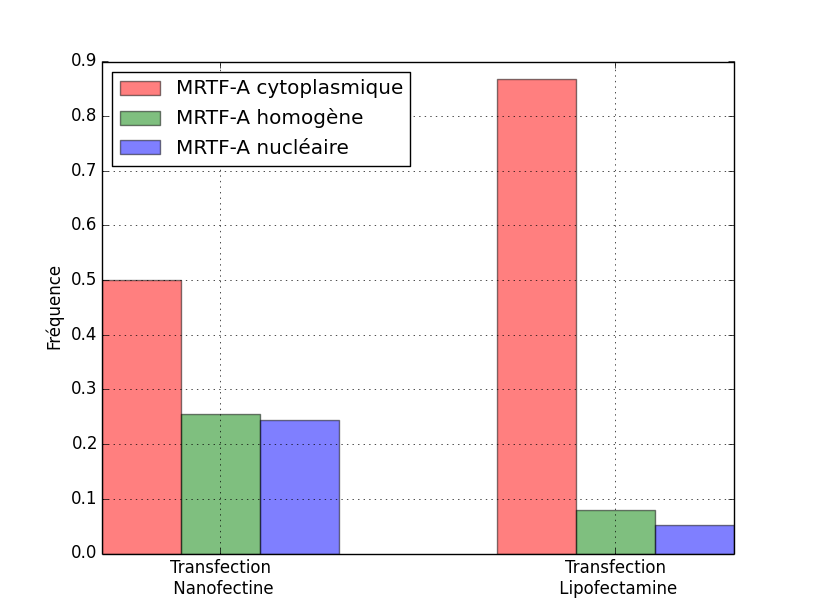
\includegraphics[scale=0.5]{Figures/Lipo_vs_Nano.png}
\caption{Comparaison de l'état après 20 minutes d'étirement (dont nous avons vu précédemment qu'il est proche de l'état initial) pour des C2C12 étirées à 10\% transfectées à la nanofectine (90 cellules en 5 expériences) ou à la lipofectamine (70 cellules en 4 expériences).  \label{LipoNano}}
\end{figure}

La figure \ref{LipoNano} montre la différence entre les répartitions initiales pour les cellules transfectées à la nanofectine et celles transfectées à la lipofectamine. On voit que MRTF-A est beaucoup plus souvent localisée dans le cytoplasme avec la lipofectamine. Cela correspond bien à ce qui est visible pendant les expériences : avec la lipofectamine, on trouve plus de cellules exprimant le plasmide, mais le niveau de fluorescence est moins fort pour chacune. Les cellules pour lesquelles la transfection a réussi sur-expriment donc moins MRTF-A GFP que lors d'une tranfection à la nanofectine.

\begin{figure}
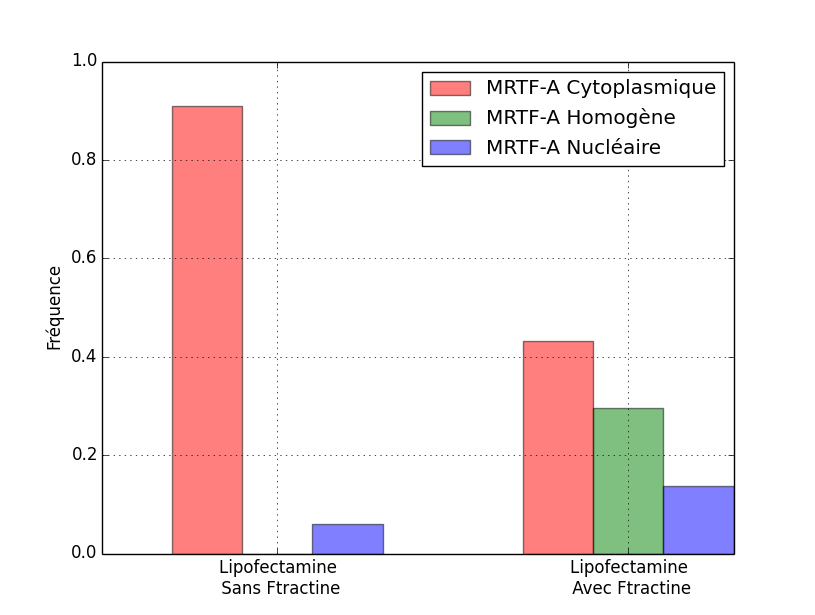
\includegraphics[scale=0.4]{Figures/Ftractine.png} 
\caption{Population initiale de cellules ayant MRTF-A cytoplasmique, homogène ou nucléaire, pour des C2C12 d'une même expérience, transfectées MRTF-A GFP et exprimant ou non la F-tractin RFP. \label{Ftractin}}
\end{figure}

On peut voir sur la figure \ref{Ftractin} que la F-tractin perturbe de manière importante la répartition de MRTF-A dans les cellules, et ce dès le début de l'observation. 
La quantité de cellules ayant MRTF-A cytoplasmique est divisée par deux dès le début de l'expérience. 


\subsubsection{Utilisation de SiRactine}
La SiRactine est un dérivé d'une drogue connue pour stabiliser les filaments d'actine, le jasplakinolide, couplé à un fluorophore dont la fluorescence sera 100 fois plus élevée lorsqu'elle est liée aux filaments d'actine. 
Elle a l'avantage de s'utiliser en très petites quantités, et directement sur les cellules à observer sans transfection et sans rinçage, ce qui fait que contrairement à l'actine mCherry ou à la LifeAct, toutes les cellules seront marquées à des niveaux semblables. 

Durant ces expériences, nous avons réalisé des mesures quantitatives d'intensité de fluorescence en MRTF-A GFP et en SiRactine. Pour chaque cellule, on calcule le ratio entre l'intensité médiane de fluorescence dans la zone péri-nucléaire et dans le noyau. Un ratio au-dessus de 1 correspond à une cellules qui était labellisée cytoplasmique, tandis qu'un ratio inférieur à 1 correspond à une localisation majoritairement nucléaire. 






La figure \ref{CHN_SiR} montre l'évolution de ces trois populations au cours du temps lors d'une expérience d'étirement 10\% avant laquelle les cellules avaient été marquées à la SiRactine. 
On peut y voir à partir de 20 minutes après étirement une diminution du nombre de cellules ayant MRTF-A dans le cytoplasme et une augmentation des localisations homogène et nucléaire simultanées, pendant environ 20 minutes. 
Cette diminution correspond à un pic des évènements C $\rightarrow H$ visible sur la figure \ref{transloc_Sir}. 
Sur la figure \ref{Siractine_quantif}, on peut constater que l'intensité de fluorescence en SiRactine croît pendant cette période de temps, indiquant une polymérisation de l'actine. 

Cette accumulation est suivie d'un plateau entre 40 et 60 minutes après l'étirement : la polymérisation de l'actine semble s'arrêter, tandis qu'en même temps le ratio moyen du signal MRTF-A GFP péri-nucléaire/nucléaire stagne et il y a un arrêt total des évènements de changement de localisation. 

À 60 minutes, la polymérisation d'actine reprend, et on peut voir qu'elle est suivie d'un pic de relocalisations de MRTF-A du cytoplasme vers le noyau (évènements C $\rightarrow$ H ) en retard d'environ 20 minutes par rapport à la reprise de la polymérisation. 

Non seulement ces expériences confirment que la relocalisation de MRTF-A vers le noyau en réponse à l'étirement est précédée de polymérisation d'actine, mais elles nous donnent également un temps de réponse, estimé à 20 minutes, entre le début de la polymérisation et l'effet visible sur MRTF-A GFP. Cela explique pourquoi pendant les expériences précédentes, presque aucune différence n'était observée entre l'état initial et l'état à 20 minutes d'étirement.

Les expériences sont en cours pour réaliser des expériences témoins transfectées à la lipofectamine, étirées mais sans marquage Siractine, et des témoins transfectées à la lipofectamine, non étirées avec marquage Siractine, afin de contrôler l'effet qu'a l'ajout de Siractine sur la polymérisation et sur la localisation de MRTF-A. 
En comparant avec les expériences précédentes transfectées à la nanofectine, on peut constater que le pic d'entrées C $\rightarrow$ H visible à 20 minutes est présent dans les deux conditions, mais qu'il est plus précoce pendant l'expérience avec SiRactine. Les deux expériences témoins devraient nous permettre de savoir si l'effet est dû au changement de méthode de transfection ( qui change la quantité de MRTF-A GFP sur-exprimée) ou à l'ajout de Siractine (qui pourrait stabiliser les filaments, par effet du jasplakinolide). 
 

\begin{figure}
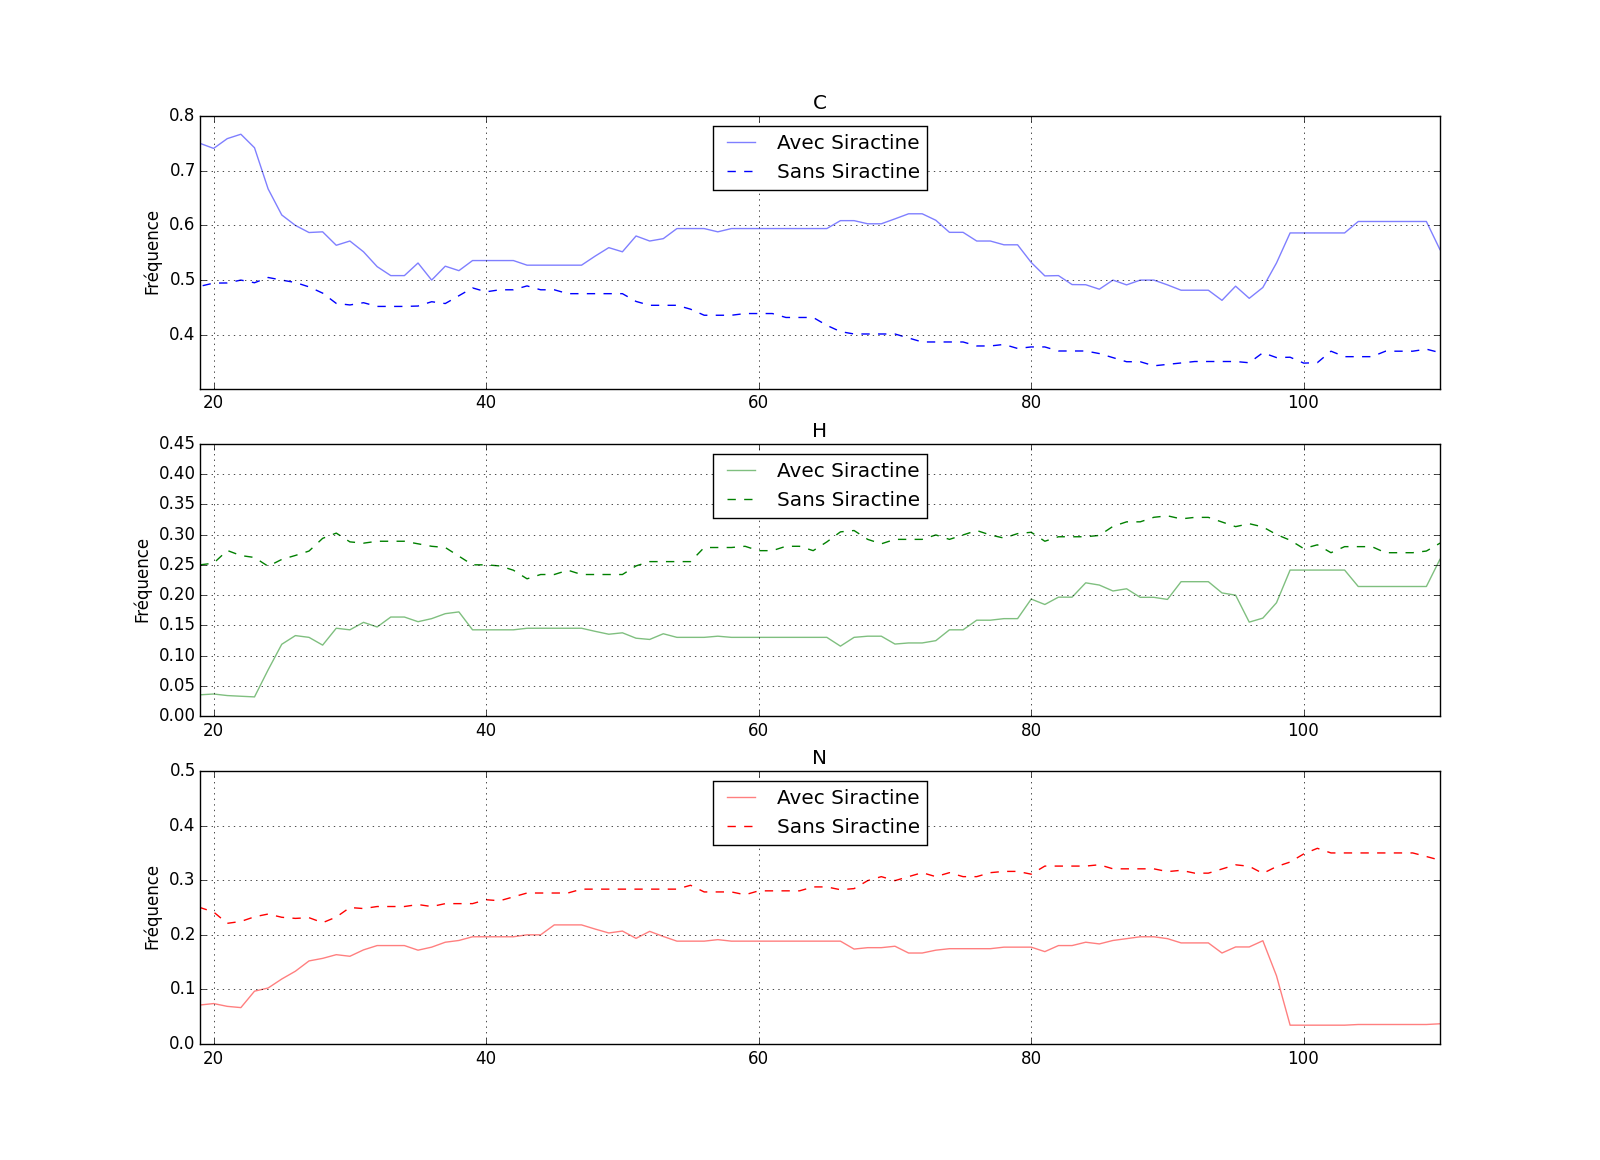
\includegraphics[scale=0.3]{Figures/Et10_Siractine_comparaison.png}
\caption{\'Evolution de la population de cellules ayant MRTF-A cytoplasmique, homogène ou nucléaire en fonction du temps écoulé depuis le début de l'étirement à 10\%, pour des C2C12 transfectées MRTF-A GFP avec de la nanofectine, et pour des C2C12 transfectées MRTF-A GFP avec de la lipofectamine et avec ajout de SiRactine pour visualiser les filaments d'actine. \label{CHN_SiR}}
\end{figure}

\begin{figure}
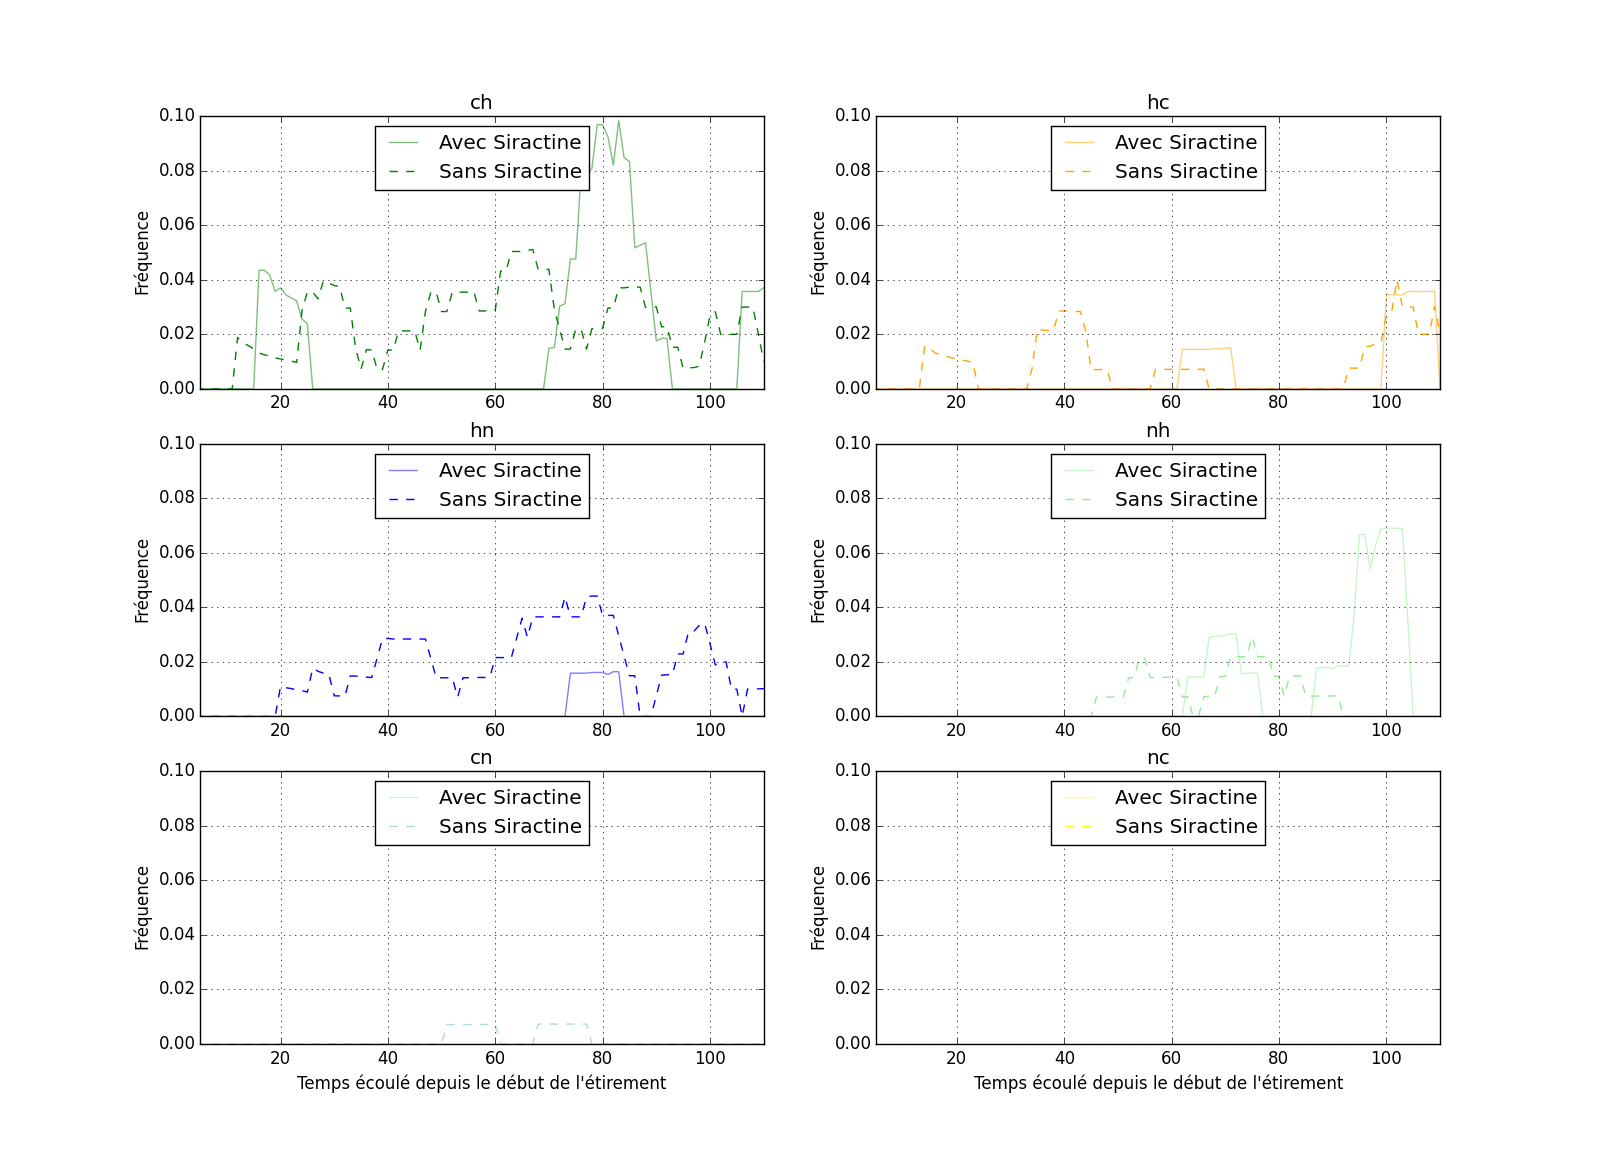
\includegraphics[scale=0.3]{Figures/Et10_transloc_Siractine.png} 
\caption{Nombre d'évènements ayant eu lieu pendant la fenêtre [t-5min,t+5min] pour chaque type de transition possible divisé par le nombre de cellules observées, pour des C2C12 transfectées MRTF-A GFP à la nanofectine et pour des C2C12 transfectées MRTF-A GFP à la lipofectamine et avec ajout de SiRactine, toutes étirées à 10\%. \label{transloc_Sir}}
\end{figure}

\begin{figure}
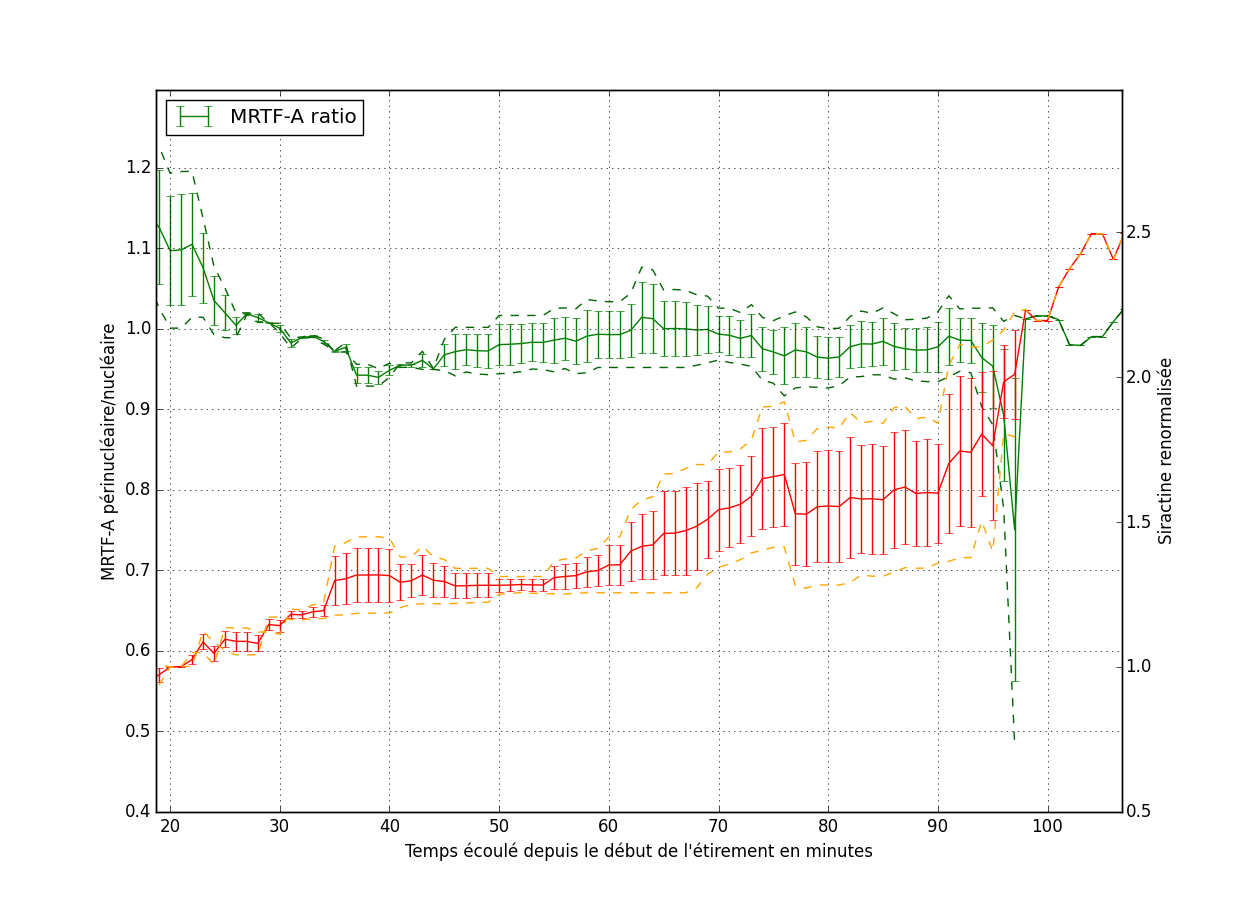
\includegraphics[scale=0.4]{Figures/C2C12.png} 
\caption{Ratio des intensités médianes de MRTF-A GFP péri-nucléaire/nucléaire (en vert) et Intensité médiane de SiRactine renormalisée par l'intensité médiane à 20 minutes (en rouge)  en fonction du temps écoulé depuis le début de l'étirement 10 \% (2 expériences, 68 cellules, les tracés en poitillés représentent chacune des deux expériences).\label{Siractine_quantif}}
\end{figure}
 


\subsection{Comparaison avec des expériences sur des myoblastes primaires}

Le travail que j'ai présenté dans ce chapitre fait partie d'un projet plus important sur le rôle de MRTF-A dans la mécanotransduction des cellules musculaires. Alessandra Pincini, post-doc à l'Institut Cochin et au laboratoire Matière et Systèmes Complexes, a pour projet de mener des expériences similaires à celles que j'ai présentées sur les C2C12, mais avec des lignées de myoblastes primaires et des myotubes différenciés à partir de ces lignées. Pour cela, elle a conçu des lentivirus avec lesquels elle a infecté ces myoblastes primaires avec la MRTF-A GFP. Elle a créé ainsi plusieurs lignées de myoblastes qui expriment de manière stable MRTF-A GFP, et qu'elle peut différencier pour créer des myotubes fluorescent. 

Durant la fin de ma thèse, afin de créer un tout cohérent avec les deux projets, Tiana Jacquemart, stagiaire de M1 au laboratoire MSC, a réalisé, avec l'aide d'Alessandra et la mienne, des expériences similaires à celles présentées à la section précédente, mais avec les myoblastes infectés créés par Alessandra Pincini. 

Les myoblastes primaires adhèrent mal au PDMS recouvert de fibronectine qui était utilisé pour les C2C12, ils sont cultivés sur des lamelles de Flexcell (Flexcell International Corporation) recouverts de collagène I. 
Ils sont ordinairement cultivés dans un milieu beaucoup plus riche en facteurs de croissance que les C2C12 (voir les détails au chapitre 6). 
Dans ces conditions, ils sont très motiles, et complètement insensibles à l'étirement du substrat. 
Afin de les amener dans des conditions plus proches des C2C12, leur milieu de culture habituel a été remplacé la veille des expériences par le milieu de culture utilisé pour les C2C12. 

\begin{figure}
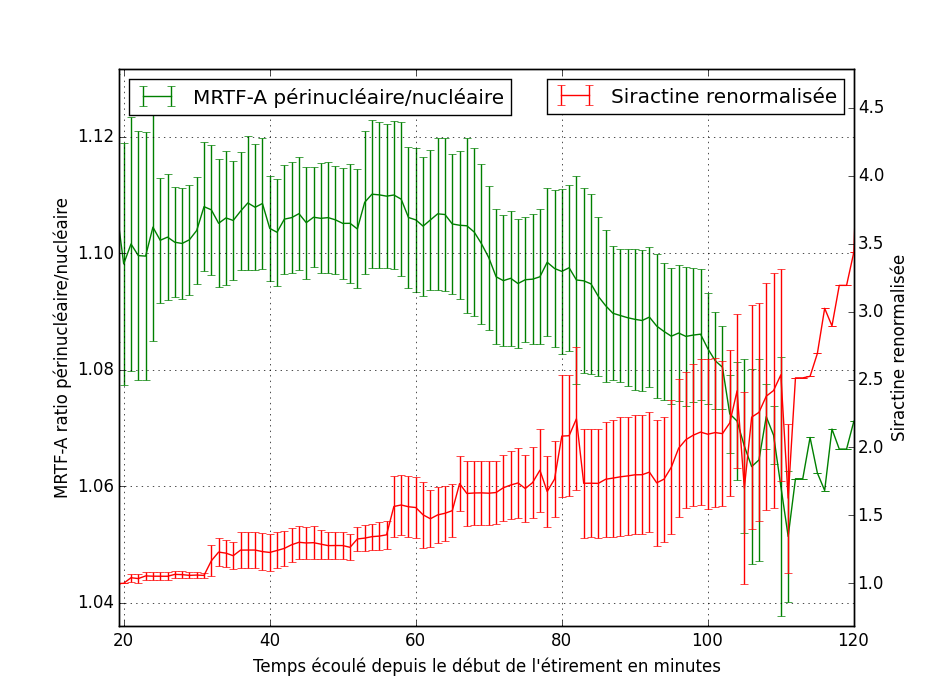
\includegraphics[scale=0.4]{Figures/Siractine_MRTFA_vs_temps.png} 
\caption{Rapport des intensités médianes en MRTF-A GFP  péri-nucléaire/nucléaire et Intensité en Siractine normalisée en fonction du temps écoulé depuis le début de l'étirement pour des myoblastes primaires soumis à 10\% d'étirement (5 expériences, 159 cellules). \label{myoblastes_Sir}}
\end{figure}

La SiRactine a une évolution proche de celle observée précédemment pour les C2C12 primaires, mais avec une croissance plus régulière au cours du temps (voir la figure \ref{myoblastes_Sir}). On peut en revanche constater que la dynamique de MRTF-A est différente : il faut attendre beaucoup plus longtemps après le début de la polymérisation pour avoir un effet sur la localisation de MRTF-A. 

Après une heure d'étirement et de polarisation, le MRTF-A ratio diminue, ce qui signifie que la part de MRTF-A qui se trouve dans le noyau augmente. 
On a donc bien à nouveau une accumulation nucléaire de MRTF-A en réponse à un signal mécanique qui active la polymérisation d'actine. 

\begin{figure}
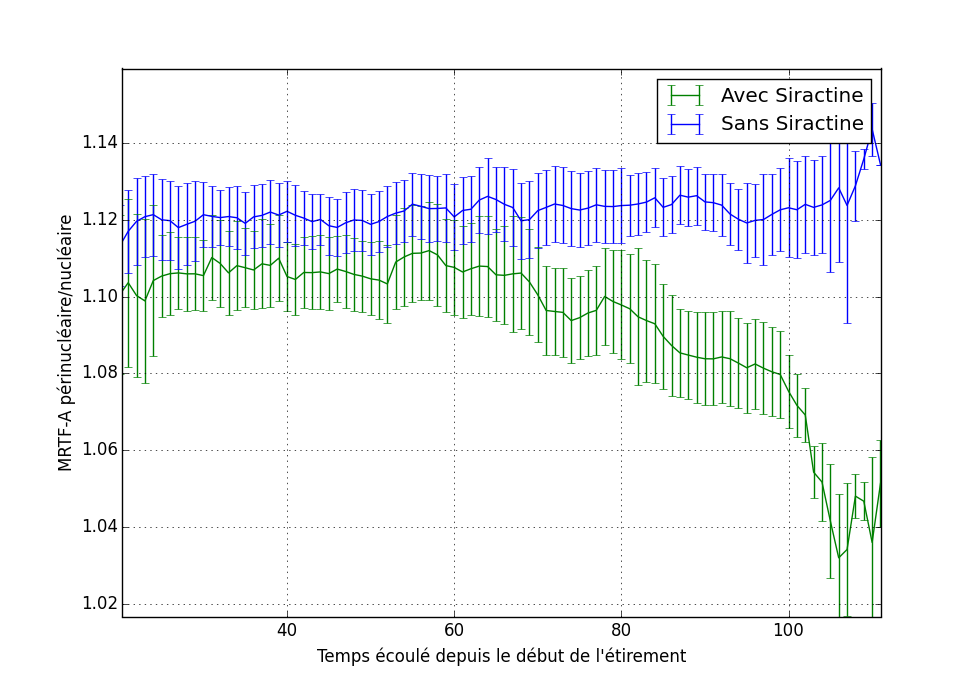
\includegraphics[scale=0.4]{Figures/Avec_Sans_Siractine.png} 
\caption{Rapport des intensités médianes en MRTF-A GFP  péri-nucléaire/nucléaire en fonction du temps écoulé depuis le début de l'étirement pour des myoblastes primaires soumis à 10\% d'étirement avec et sans ajout de SiRactine (Avec SiRactine : 5 expériences, 159 cellules, Sans SiRactine : 5 expériences, 239 cellules)}
\end{figure}

Cependant, un contrôle réalisé avec des myoblastes primaires non marqués avec la SiRactine nous montre une absence d'accumulation nucléaire de MRTF-A en réponse à l'étirement. 
Dès le début de l'expérience, on peut voir que le MRTF-A ratio moyen est plus élevé sans SiRactine qu'avec. 
La SiRactine est un dérivé d'une drogue connue pour stabiliser les filaments d'actine, il est donc raisonnable de supposer que l'ajout, même d'une quantité aussi faible (2,5nM), de Siractine, puisse augmenter la quantité de filaments d'actine dans la cellule au détriment des monomères, et contribuer à plus de MRTF-A dans le noyau. 
La différence entre les deux expériences pourrait alors s'expliquer ainsi : la SiRactine augmente la quantité de filaments par rapport aux monomères, elle déplace donc l'équilibre entre MRTF-A et la G-actine plus proche du point où il y a trop de MRTF-A et pas assez de G-actine.
Lorsque l'étirement est imposé, il y a polymérisation de l'actine dans les deux cas, mais c'est seulement dans le cas où le ratio F-actine/G-actine est déjà élevé que l'augmentation suffit à faire basculer l'équilibre chimique de la cellule en faveur d'une MRTF-A libre de rentrer dans le noyau. 

Des expériences témoins sans étirement, avec ou sans SiRactine sont également en cours pour essayer de déterminer ce qui relève de l'effet de l'étirement et ce qui relève de l'ajout de SiRactine, en particulier pour vérifier que l'augmentation d'intensité de la SiRactine est bien liée à l'application de l'étirement. 

La SiRactine s'est révélée un outil très efficace d'observation en direct de l'actine. Cependant, l'équilibre de MRTF-A GFP est suffisamment sensible pour détecter son influence même à de très faibles concentrations. 
Les marquages sur cellules fixées ont cet avantage de ne pas perturber les cellules, puisque les marqueurs sont ajoutés après la fin de la vie de la cellule. 
Ils nous permettent également de marquer la G-actine en plus de la F-actine, ce qui ne nous est actuellement pas possible sur des cellules vivantes. 


\section{Application d'une déformation globale avec l'étireur : \'Etude quantitative sur cellules fixées}

Lors de ces expériences, des cellules transfectées MRTF-A GFP étaient ensemencées sur 6 lamelles de PDMS. Puis chacune d'elle était successivement montée dans l'étireur, étirée à 10 ou 30 \%, puis laissée en étirement à l'incubateur pendant un temps donné. Une fois le temps écoulé, la lamelle était démontée et fixée. Après fixation, l'actine F, l'actine G et le noyau étaient marqués , et les lamelles étaient observées en microscopie de fluorescence. Le protocole de l'étirement et du marquage sont décrits en détail dans le chapitre dédié aux méthodes expérimentales. 
Trois expériences indépendantes sur des cellules MRTF-A GFP ont été réalisées pour chacun des deux étirements possibles. Une expérience sur des cellules non transfectées, mais marquées avec un anti-corps MRTF-A, a été réalisée pour chaque étirement. 

Initialement, l'un des objectifs était de pouvoir quantifier l'évolution de la quantité de F-actine par rapport à celle de G-actine. Cependant, il est apparu à la fin de la série d'expériences que l'intensité de fluorescence de la phalloïdine était de moins en moins fiable avec le temps. Les expériences réalisées immédiatement après l'ouverture du flacon de phalloïdine, qui comprennent les trois expériences d'étirement 30 \% et une seule expérience à 10\%, sont exploitables. Dans les expériences réalisées plus tard, au mois d'avril 2014, la phalloïdine devient beaucoup plus sensible au photo-blanchiment, et l'ordre dans lequel les lamelles sont observées est le déterminant majeur de l'intensité de fluorescence observée, ce qui fausse complètement les observations. 
Pour palier à cet effet, pour les expériences du mois de juin 2014 qui concernent les cellules non transfectées, toutes les lamelles ont été observées le même jour et pendant des durées bien inférieures, afin de réduire l'influence du phénomène. 

\subsection{Résultats pour l'étirement 10\% : expulsion de la G-actine hors du noyau}

Pendant les expériences étirées à 10\% en direct, on avait pu observer une tendance nette à l'accumulation de MRTF-A GFP dans le noyau des cellules. 

\begin{figure}
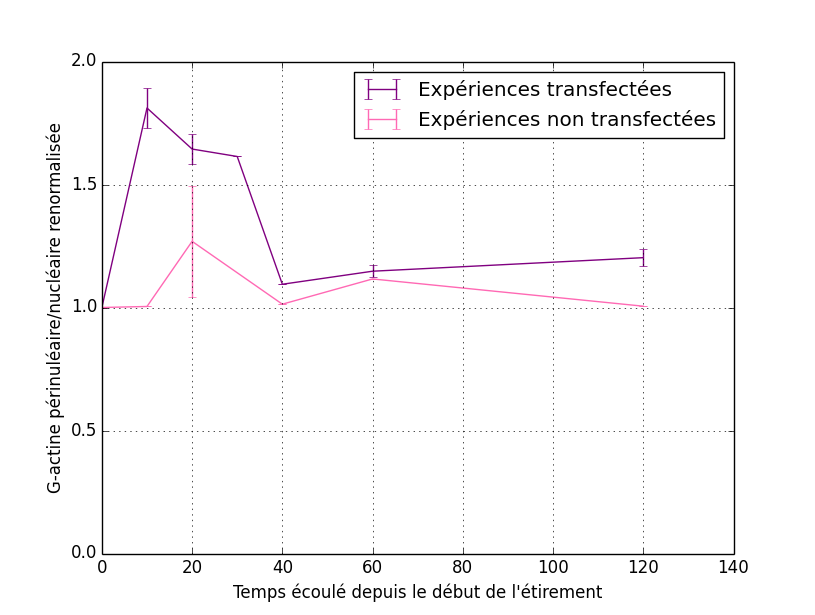
\includegraphics[scale=0.5]{Figures/Et10_G_ratio.png} 
\caption{\label{Et10_G} Intensité médiane du signal en DNase I (G-actine) dans la zone périnucléaire par rapport à la zone nucléaire, pour deux expériences sur des cellules MRTF-A GFP et deux expériences sur des cellules MRTF-A endogène, étirées à 10\%. Les données sont normalisées par la valeur au temps t=0, pour enlever les variations dues à la qualité du marquage d'une expérience à l'autre.}
\end{figure}

L'observation la plus frappante de ces expériences concerne la localisation de l'actine monomérique dans la cellule. En effet, on peut constater sur la figure \ref{Et10_G} pour quatre expériences indépendantes que la quantité d'actine monomérique dans le noyau semble décroître brutalement par rapport à l'actine monomérique dans le cytoplasme, entre 10 et 20 minutes après le début de l'étirement, avant de retrouver sa localisation initiale. Cela ressemble à une expulsion massive des monomères d'actine hors du noyau. 

Ce résultat peut paraître contre-intuitif : comment cette expulsion d'actine hors du noyau, qui diminue notablement le ratio F/G peut-il permettre l'accumulation nucléaire de MRTF-A ? En réalité, il existe deux manière pour la cellule de confiner MRTF-A dans le noyau. La première est liée au manque de G-actine dans le cytoplasme, qui va conduire à l'import rapide de MRTF-A. La seconde est liée au manque de G-actine dans le noyau, qui va empêcher MRTF-A de sortir du noyau, car cette dernière a besoin de se lier à la G-actine pour être exportée. Ici c'est donc le manque de G-actine dans le noyau qui conduit à l'accumulation de MRTF-A GFP. 

Or récemment, il a été montré que la protéine MICAL-2, présente majoritairement dans le noyau, est capable, en réponse au sérum, de dépolymériser les filaments d'actine en oxydant les monomères qui le compose \cite{lundquist_redox_2014}. De plus, ces monomères d'actine oxydée sont expulsés du noyau. De plus, MICAL-2 a également été lié à l'accumulation d'actine dans le noyau et l'exclusion de MRTF-A dans le cytoplasme des cellules musculaires lors de l'atrophie provoquée par une dénervation chez la souris \cite{collard_nuclear_2014}. MICAL-2 apparaît donc comme une piste sérieuse pour expliquer l'expulsion massive d'actine monomérique hors du noyau suite à l'application de l'étirement. 

De manière encore inexpliquée pour l'instant, une des expériences avec des cellules non transfectées ne montre pas cet effet sur l'actine monomérique autour de 10 à 20 minutes d'étirement. Tout au plus peut-on observer une augmentation du ratio de G-actine péri-nucléaire par rapport à nucléaire au bout de 40 minutes. Une des pistes pourrait être la quantité de DMEM plus importante mise dans chaque puits, à concentration égale, pour les besoins de cette expérience , qui mènerait à une plus grande concentration en sérum le lendemain de l'expérience. La concentration en sérum et la quantité d'actine monomérique ont en effet déjà été liées dans d'autres expériences \cite{mouilleron_molecular_2008},\cite{vartiainen_nuclear_2007}\cite{lundquist_redox_2014}.  



\subsection{Résultats pour l'étirement 30\% : une dépolymérisation des filaments d'actine dans le cytoplasme}

Les résultats des expériences à 30\% d'étirement pointaient vers une dépolymérisation brutale du cytosquelette d'actine en réponse à l'étirement. 

\begin{figure}
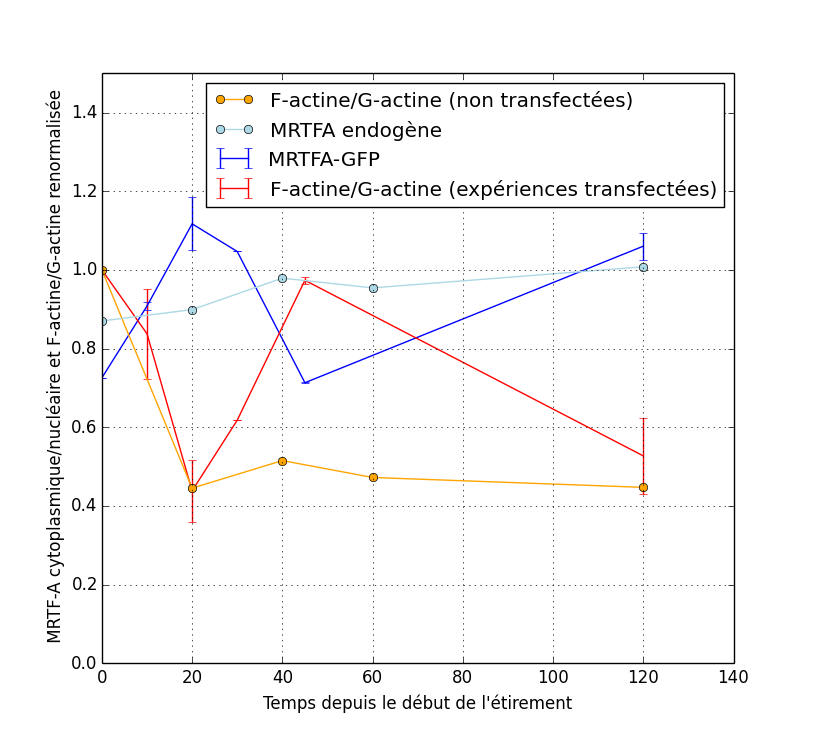
\includegraphics[scale=0.5]{Figures/Et30_MRTFA_FG.png} 
\caption{\label{Et30_MRTFA_FG} Intensité médiane de MRTFA-GFP ou de MRTF-A endogène dans la zone péri-nucléaire par rapport à la zone nucléaire (en bleu) et intensité médiane de la phalloïdine (F-actine) par rapport à la DNaseI (G-actine) (en rouge et orange)  au cours du temps, pour trois expériences transfectées et une non tranfectée, étirées à 30\%.  }
\end{figure}
\begin{figure}
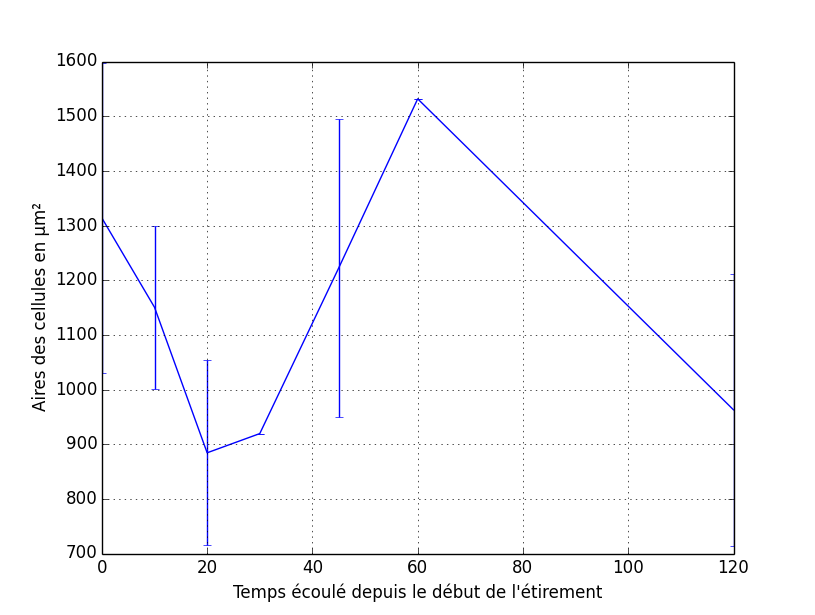
\includegraphics[scale=0.5]{Figures/Et30_Aires.png} 
\caption{\label{Et30_Aires} Aire moyenne des cellules au cours du temps pendant l'étirement 30\%. }
\end{figure}
Ces résultats sont confirmées par les expériences, tant en MRTF-A GFP qu'en MRTF-A endogène. On peut constater sur la figure \ref{Et30_MRTFA_FG} que 20 minutes après le début de l'étirement la proportion d'actine F par rapport à l'actine G est diminuée de moitié. Cette diminution est accompagnée d'une diminution de l'aire des cellules visible sur la figure \ref{Et30_Aires}. Cela confirme que les cellules ne peuvent pas supporter des déformations aussi importantes, en conséquence de quoi elles se décollent et leur réseau d'actine est dépolymérisé. 

La dépolymérisation est suivie d'une récupération qui se fait à un rythme variable d'une expérience à l'autre, sans que l'on ait pour l'instant réussi à distinguer l'origine de cette variabilité. 

On constate également que l'expulsion de l'actine monomérique du noyau est présente mais de manière beaucoup moins marquée que lors de l'étirement 10 \%. Cela pourrait signifier que la même voie que pour l'étirement 10 \% est activée, mais que son action est diminuée et masquée par les dommages causés au cytosquelette, jusqu'au moment où la récupération a eu lieu. 


\section{Synthèse des résultats expérimentaux}

Durant cette thèse, nous avons observé l'effet de deux types de contraintes mécaniques, locales avec les pinces magnétiques et globales avec l'étirement du substrat, sur la localisation de la protéine MRTF-A et sur l'état du cytosquelette d'actine dans des myoblastes. 
Il en ressort clairement que l'application d'une contrainte induit une polymérisation de l'actine, qui précède une relocalisation de MRTF-A du cytoplasme vers le noyau des cellules. Lorsque la contrainte est plus élevée, le cytosquelette d'actine peut être abimé, et subir une dépolymérisation partielle qui s'accompagne d'une relocalisation très rapide de MRTF-A vers le cytoplasme. 

Ces deux résultats sont tout à fait cohérent avec les résultats déjà publiés à propos des mécanismes de régulation de la localisation de MRTF-A par l'actine présentés dans le chapitre 3 : lorsque l'actine polymérise, il n'y a plus assez de monomères d'actine pour se lier à MRTF-A, et celle-ci est libre d'être transportée vers le noyau. Tant qu'il y a peu de monomères d'actine dans le noyau, elle y est séquestrée. Au contraire, lorsque beaucoup de monomères d'actine sont disponibles pour se lier à MRTF-A (comme dans le cas de la dépolymérisation à grand étirement), celle-ci est éjectée du noyau et séquestrée dans le cytoplasme. 

On a également pu voir que tout perturbation de l'équilibre entre les filaments et les monomères d'actine a une influence visible sur la localisation de MRTF-A. Lorsque l'actine est sur-exprimée, l'abondance de monomères disponibles maintient MRTF-A dans le cytoplasme et bloque tout effet de l'étirement. Au contraire, lorsque la LifeAct, la F-tractine ou la SiRactine favorisent la stabilité des filaments, MRTF-A s'accumule plus souvent dans le noyau, et l'effet des stimulations mécaniques est augmenté. Enfin, nous avons pu voir que même un changement minime de concentration de sérum comme le rinçage peut suffire à perturber la localisation de MRTF-A. Bien que l'effet du sérum ait été abondamment décrit dans la littérature, il s'agissait de changements important de concentration. Nous avons montré ici qu'il faut être attentif à la moindre perturbation de l'équilibre entre filaments et monomères d'actine, que ce soit pas les marqueurs du cytosquelette ou par le sérum, lorsque l'on souhaite étudier MRTF-A. 

Le début des expériences sur les myoblastes primaires fait le pont entre ce qui a été montré sur les C2C12 et les expériences que mène Alessandra Pincini sur les myotubes, qui sont des cellules beaucoup plus proches de l'organisation des cellules musculaires matures. 
Nous avons constaté sur elles le même effet perturbateur de la SiRactine, mais leur comportement en réponse à l'étirement n'est pas tout à fait le même que celui des C2C12. 
À terme, des expériences allant des myoblastes aux myotubes viendront compléter l'espace entre les expériences \textit{in vitro} sur les C2C12 et les expériences \textit{in vivo} sur les souris de \cite{guerci_srf-dependent_2012} et \cite{collard_nuclear_2014}, pour former une image complète du rôle de MRTF-A dans les cellules musculaires. 

Enfin, les changements de localisation de l'actine monomérique, qui est exclue du noyau lors de l'étirement sur les cellules fixées, est un nouvel élément intriguant de la régulation de MRTF-A. La récente arrivée de MICAL-2  (\cite{lundquist_redox_2014},\cite{collard_nuclear_2014}) et et de la polymérisation de l'actine nucléaire \parencite{baarlink_nuclear_2013} dans les acteurs de la régulation de MRTF-A sont des pistes pour expliquer ces observations. Une régulation de MRTF-A à deux éléments commence à se dessiner avec ces dernières expériences : un premier mécanisme organise la polymérisation des filaments et donc l'appauvrissement en G-actine dans le cytoplasme qui sont nécessaires pour faire entrer MRTF-A dans le noyau, tandis qu'un second mécanisme dépendant de MICAL-2 organise l'expulsion de l'actine du noyau pour empêcher MRTF-A de sortir du noyau. Les deux mécanismes se complètent alors pour s'assurer que MRTF-A entre dans le noyau et ne puisse pas en ressortir, conduisant à une accumulation de longue durée de MRTF-A dans le noyau.
De nouvelles expériences, en particulier avec les SiRNA anti-MICAL-2 qui viennent d'être développés par Alessandra Pincini, permettront d'explorer ces nouvelles pistes. 








%\end{document}